%------------------------------------------------------------------------------
\section{Foundations of Reinforcement Learning}
\label{sec:foundations}
%------------------------------------------------------------------------------

This section establishes the foundational concepts and notation that 
underpin the remainder of this dissertation. Beginning with the classical 
formulation of sequential decision-making under uncertainty, we trace 
the development of \gls{rl} from tabular methods through function 
approximation to the deep learning revolution that enabled modern applications. 
The section concludes with a detailed examination of \gls{ppo}, 
the algorithm used in all three contributions of this dissertation.

\subsection{Single-Agent Reinforcement Learning}
\label{sec:single-agent-rl}

\Gls{rl} addresses the problem of an agent learning to make sequential decisions 
through interaction with an environment to maximize cumulative reward \cite{sutton2018}. 
Unlike supervised learning, where explicit input-output pairs guide the learning process, 
\gls{rl} agents must discover effective behaviors through trial and error, 
balancing the exploration of unknown actions against the exploitation of 
known rewards \cite{kaelbling1996}.

\subsubsection{Markov Decision Processes}
\Glspl{mdp} form the foundation of reinforcement learning by providing 
a formal framework for modeling decision-making in environments with 
stochastic dynamics~\cite{puterman2005}. An \gls{mdp} is defined by a tuple 
(\Gls{s}, \Gls{a}, \gls{P}, \gls{rew}, \gls{discount}), where:
\begin{itemize}
    \item \Gls{s} is a finite set of states.
    \item \Gls{a} is a finite set of actions.
    \item \(\gls{P}: \Gls{s} \times \Gls{a} \times \Gls{s} \rightarrow [0,1]\) is the state 
        transition probability function, where \(P(\gls{s}^\prime|\gls{s}, \gls{a})\) 
        represents the probability of transitioning to state \(\gls{s}^\prime\in \Gls{s}\)
        given the current state \(\gls{s}\in \Gls{s}\) and action \(\gls{a}\in \Gls{a}\).
        This captures the stochastic nature of the environment.
    \item \(\gls{rew}: \Gls{s} \times \Gls{a} \rightarrow \gls{reals}\) is the reward 
        function and written as \(R(\gls{s}, \gls{a})\) defines the immediate reward 
        received after taking action \(\gls{a}\in \Gls{a}\) in state \(\gls{s}\in \Gls{s}\). 
        This reward guides the agent's learning process.
    \item \(\gls{discount} \in [0, 1]\) is the discount factor, which 
        determines the level of importance given to estimated future rewards. 
        Specifically, \(\gls{discount}=1\) implies that a reward estimate is 
        given equal value regardless of how many steps in the future it may 
        be while \(\gls{discount}=0\) implies that only the value of a 
        reward in the next step is considered.
\end{itemize}

\begin{figure}
    \centering
    \input{mdp_cycle}
    \caption{\glsentryshort{rl} exemplified by a 
        fully reduced \glsentryshort{mdp}.}
    \label{fig:mdp_cycle}
\end{figure}

A common depiction of reinforcement learning illustrates it as a simple 
feedback loop between an agent and its environment. In its most basic form, 
this process can be modeled as a fully reduced \gls{mdp}, where the agent observes
the state, selects an action, and receives a reward from the environment in response. 
\Cref{fig:mdp_cycle} highlights this alternating cycle, often referred to as the 
\emph{training loop}.

The Markov property asserts that the future state depends only on the current 
state and action, not on the history of prior states: 
\(
    \gls{p}(\gls{s}_{\gls{t}+1} | \gls{s}_{\gls{t}}, \gls{a}_{\gls{t}}, 
    \gls{s}_{\gls{t}-1}, \gls{a}_{\gls{t}-1}, \ldots) 
    = \gls{p}(\gls{s}_{\gls{t}+1} | \gls{s}_{\gls{t}}, \gls{a}_{\gls{t}})
\). 
This memoryless property enables tractable computation while 
remaining sufficiently expressive to model a wide range of decision problems.

A policy \(\gls{pi}: \mathcal{\Gls{s}} \rightarrow \Delta(\mathcal{\Gls{a}})\) maps 
states to probability distributions over actions, where \(\gls{pi}(\gls{a}|\gls{s})\) 
denotes the probability of selecting action \(\gls{a}\) in state \(\gls{s}\). 
The agent's objective is to find an optimal policy \(\gls{pi}^*\) that maximizes 
the expected discounted return:
\begin{equation}
    \gls{pi}^* = \arg\max_{\gls{pi}} \gls{expRet}_{\gls{pi}} \left[ \sum_{\gls{t}=0}^{\infty} 
        \gls{discount}^{\gls{t}} \Gls{r}(\gls{s}_{\gls{t}}, \gls{a}_{\gls{t}}) \right]
\end{equation}

\subsubsection{Value Functions and Optimality}

Central to RL are value functions, which estimate the expected return 
from a given state or state-action pair under a particular policy. 
The state value function \(\Gls{v}_{\gls{pi}}\) represents the expected return 
starting from state \(\gls{s}\) and following policy \(\gls{pi}\):
\begin{equation}
    \Gls{v}_{\gls{pi}} = \gls{expRet}_{\gls{pi}} \left[ \sum_{\gls{t}=0}^{\infty} 
        \gls{discount}^{\gls{t}} \Gls{r}(\gls{s}_{\gls{t}}, \gls{a}_{\gls{t}}) 
        \mid \gls{s}_0 = \gls{s} \right]
\end{equation}

Similarly, the action-value function \(\Gls{q}_{\gls{pi}}(\gls{s},\gls{a})\) captures 
the expected return of taking action $a$ in state $s$ and subsequently following \(\gls{pi}\):
\begin{equation}
    \Gls{q}_{\gls{pi}}(\gls{s}, \gls{a}) = \gls{expRet}_{\gls{pi}} \left[ \sum_{\gls{t}=0}^{\infty}
        \gls{discount}^{\gls{t}} \Gls{r}(\gls{s}_{\gls{t}}, \gls{a}_{\gls{t}}) 
        \mid \gls{s}_0 = \gls{s}, \gls{a}_0 = \gls{a} \right]
\end{equation}

These functions satisfy the Bellman equations, recursive relationships that 
decompose the value of a state into immediate reward and discounted future value. 
The Bellman optimality equations characterize the optimal value functions 
\(\Gls{v}^*\) and \(\Gls{q}^*\), from which optimal policies can be derived \cite{sutton2018}.

Q-learning, introduced by \cite{watkins1992}, provides a model-free method for learning 
\(\Gls{q}^*\) directly from experience without requiring knowledge of the transition dynamics. 
The algorithm updates \(\Gls{q}\)-values toward a target that combines the observed reward 
with the maximum estimated future value:
\begin{equation}
    \Gls{q}(\gls{s}_{\gls{t}}, \gls{a}_{\gls{t}}) \leftarrow 
    \Gls{q}(\gls{s}_{\gls{t}}, \gls{a}_{\gls{t}}) + \gls{step} \left[ \gls{r}_{\gls{t}} 
        + \gls{discount} \max_{\gls{a}'} \Gls{q}(\gls{s}_{\gls{t}+1}, \gls{a}') 
        - \Gls{q}(\gls{s}_{\gls{t}}, \gls{a}_{\gls{t}}) \right]
\end{equation}
where \(\gls{step}\) is the learning rate. Under appropriate conditions on the learning rate 
and exploration, Q-learning converges to the optimal action-value function in tabular settings.

\subsubsection{Policy Gradient Methods}

While value-based methods like Q-learning learn a value function from which a policy is derived, 
policy gradient methods directly parameterize and optimize the policy \(\gls{pi}_{\theta}\). 
This approach offers several advantages: natural handling of continuous action spaces, 
the ability to learn stochastic policies, and often more stable learning dynamics in practice.

The policy gradient theorem provides the foundation for this class of algorithms, 
establishing that the gradient of the expected return with respect to policy 
parameters can be estimated from sampled trajectories \cite{sutton2018}:
\begin{equation}
    \nabla_\theta J(\theta) = \gls{expRet}_{\gls{pi}_\theta} \left[ 
        \nabla_\theta \log \gls{pi}_\theta(a|s) \cdot \Gls{g}_{\gls{t}} \right]
\end{equation}
where \(\Gls{g}_{\gls{t}} = \sum_{k=0}^{\infty} \gls{discount}^k \gls{r}_{\gls{t}+k}\) 
is the return from time \(\gls{t}\).

\glsunset{reinforce}
The \gls{reinforce} algorithm \cite{williams1992} provides a 
Monte Carlo implementation of this gradient estimate, 
using complete episode returns to update policy parameters. 
While unbiased, \gls{reinforce} estimates exhibit high variance, 
motivating the development of variance reduction techniques 
including baseline subtraction and actor-critic architectures.

%------------------------------------------------------------------------------
\subsection{Deep Reinforcement Learning}
\label{sec:deep-rl}
%------------------------------------------------------------------------------

Classical \gls{rl} methods rely on tabular representations that enumerate 
values for every state or state-action pair. While theoretically elegant, 
this approach becomes intractable as state spaces grow large or continuous. 
Function approximation addresses this limitation by representing value functions 
or policies as parameterized functions capable of generalizing across similar states.

\subsubsection{Function Approximation with Neural Networks}

Neural networks provide a powerful class of function approximators capable of 
representing complex, nonlinear mappings from high-dimensional inputs to outputs. 
When combined with \gls{rl}, neural networks enable agents to learn directly from raw 
sensory inputs such as images, eliminating the need for hand-crafted feature engineering.

However, the combination of function approximation with bootstrapping 
(using estimated values as targets) and off-policy learning creates the 
``deadly triad'' that can lead to divergent learning dynamics \cite{sutton2018}. 
Stabilizing deep \gls{rl} required algorithmic innovations to address these challenges.

\subsubsection{Deep Q-Networks and the Deep RL Revolution}

The \gls{dqn} introduced by \cite{mnih2013, mnih2015} demonstrated that 
neural networks could learn effective policies directly from pixel inputs, 
achieving human-level performance across a diverse suite of Atari 2600 games. 
This breakthrough relied on two key innovations: experience replay and target networks.

Experience replay stores transitions 
\((\gls{s}_{\gls{t}}, \gls{a}_{\gls{t}}, \gls{r}_{\gls{t}}, \gls{s}_{\gls{t}+1})\)
in a buffer and samples mini-batches uniformly for training, breaking the 
temporal correlation between consecutive samples that destabilizes learning. 
Target networks maintain a separate, slowly-updated copy of the Q-network 
used to compute learning targets, reducing the moving target problem inherent 
in bootstrapping.

\Gls{dqn} parameterizes the action-value function as \(\Gls{q}(\gls{s}, \gls{a}; \theta)\)
and minimizes the temporal difference error:
\begin{equation}
    \mathcal{L}(\theta) = \gls{expRet}_{(\gls{s},\gls{a},\gls{r},\gls{s}') \sim \mathcal{D}} 
    \left[ \left( \gls{r} + \gls{discount} \max_{\gls{a}'} \Gls{q}(\gls{s}', \gls{a}'; 
        \theta^-) - \Gls{q}(\gls{s}, \gls{a}; \theta) \right)^2 \right]
\end{equation}
where \(\mathcal{D}\) is the replay buffer and 
\(\theta^-\) are the parameters of the target network.

The success of \gls{dqn} catalyzed rapid progress in deep \gls{rl}, 
with subsequent work addressing its limitations. 
\Gls{ddpg} extended the approach to continuous action spaces by learning 
a deterministic policy alongside the Q-function \cite{lillicrap2019}.
\Gls{td3} further improved stability by addressing overestimation bias 
through double Q-learning and delayed policy updates \cite{fujimoto2018}.

\subsubsection{Actor-Critic Architectures}
% #OPT: Add Actor critic diagram?

Actor-critic methods combine the advantages of policy gradient and 
value-based approaches by maintaining both a policy (the actor) 
and a value function (the critic). The critic provides lower-variance 
estimates of expected returns to guide policy updates, 
while the actor enables direct policy optimization.

The \gls{a2c} algorithm uses the advantage function 
\(\Gls{a}_{\gls{pi}}(\gls{s}, \gls{a}) 
= \Gls{q}_{\gls{pi}}(\gls{s}, \gls{a}) 
- \Gls{v}_{\gls{pi}}(\gls{s})\)
to reduce variance while maintaining an unbiased gradient estimate. 
The advantage captures how much better an action is compared to the 
average action under the current policy, providing a 
natural baseline that centers the learning signal.

\Gls{a3c} introduced by \cite{mnih2016} demonstrated that parallel, 
asynchronous training across multiple environment instances could 
stabilize learning without experience replay. Multiple actors collect experience 
simultaneously while asynchronously updating a shared parameter server, 
with the diversity of experience naturally decorrelating updates.

\Gls{trpo} addressed the challenge of determining appropriate step sizes 
for policy updates \cite{schulman2017}. By constraining updates to a 
trust region defined by the KL-divergence between successive policies, 
\gls{trpo} ensures monotonic improvement guarantees while enabling larger, 
more efficient updates than vanilla policy gradients. This theoretical 
foundation directly motivated the development of \gls{ppo}.

%------------------------------------------------------------------------------
\subsection{Proximal Policy Optimization}
\label{sec:ppo}
%------------------------------------------------------------------------------

\Glsentryfull{ppo}, introduced by \cite{schulman2017a}, 
has become the predominant algorithm for both single-agent and multi-agent 
reinforcement learning due to its combination of strong empirical performance, 
implementation simplicity, and computational efficiency. 
All three contributions of this dissertation employ \gls{ppo} as the underlying 
optimization algorithm, making a detailed understanding of its mechanics essential.

\subsubsection{The Clipped Surrogate Objective}

\Gls{ppo} builds on the insight from \gls{trpo} that constraining 
policy updates improves stability, but replaces the computationally 
expensive constrained optimization with a simpler clipped objective. 
The key quantity is the probability ratio between the new and old policies:
\begin{equation}
    \gls{r}_{\gls{t}}(\theta) = \frac{\gls{pi}_\theta(\gls{a}_{\gls{t}} 
    | \gls{s}_{\gls{t}})}{\gls{pi}_{\theta_{\text{old}}}(\gls{a}_{\gls{t}} | \gls{s}_{\gls{t}})}
\end{equation}

The clipped surrogate objective prevents excessively large policy updates by 
limiting the effective change in action probabilities:
\begin{equation}
    \mathcal{L}^{\text{CLIP}}(\theta) = \gls{expRet}_{\gls{t}} \left[ 
        \min \left( \gls{r}_{\gls{t}}(\theta) \hat{\Gls{a}}_{\gls{t}}, 
        \, \text{clip}(\gls{r}_{\gls{t}}(\theta), 1-\epsilon, 1+\epsilon) 
        \hat{\Gls{a}}_{\gls{t}} \right) \right]
\end{equation}
where \(\hat{\Gls{a}}_{\gls{t}}\) is the estimated advantage at time \(\gls{t}\) and 
\(\epsilon\) is a hyperparameter (typically 0.1--0.2) controlling the clipping range.

The minimum operation ensures conservative updates: when the advantage is positive 
(the action was better than expected), the objective increases with \(\gls{r}_{\gls{t}}\)
but is clipped at \(1+\epsilon\); when the advantage is negative, 
the objective decreases with \(\gls{r}_{\gls{t}}\) but is clipped at \(1-\epsilon\). 
This mechanism discourages the policy from moving too far from the behavior that 
generated the training data, similar in spirit to the trust region constraint in
\gls{trpo} \cite{kakade2002}.

\subsubsection{Generalized Advantage Estimation}

\Gls{ppo} typically employs \gls{gae} to compute advantage estimates that 
balance bias and variance. \Gls{gae} interpolates between Monte Carlo returns 
(low bias, high variance) and one-step temporal difference estimates 
(higher bias, lower variance) through an exponentially-weighted average:
\begin{equation}
    \hat{\gls{adv}}_t^{\text{GAE}(\gls{discount}, \lambda)} 
    = \sum_{l=0}^{\infty} (\gls{discount} \lambda)^l \delta_{t+l}
\end{equation}
where \(\delta_{\gls{t}} = \gls{r}_{\gls{t}} + \gls{discount} V(s_{t+1}) 
- V(s_{\gls{t}})\) is the temporal difference residual and 
\(\lambda \in [0,1]\) controls the bias-variance trade-off.

\subsubsection{Importance for Multi-Agent Adoption}

Several properties of \gls{ppo} have driven its widespread adoption in multi-agent settings. 
First, \gls{ppo}'s on-policy nature aligns naturally with the training paradigm where 
all agents simultaneously collect experience and update policies. Second, 
the clipped objective provides stability against the non-stationarity 
introduced by simultaneously learning agents, where each agent's environment 
effectively changes as other agents' policies evolve. Third, \gls{ppo}'s sample efficiency, 
while not matching off-policy methods in single-agent settings, scales favorably when 
parallelized across multiple agents and environments.

The surprising effectiveness of \gls{ippo}, where each agent independently 
optimizes a \gls{ppo} objective without explicit coordination, has been 
empirically demonstrated across diverse cooperative benchmarks \cite{yu2022}. 
This finding suggests that PPO's implicit regularization through clipping may be 
particularly well-suited to multi-agent learning dynamics, providing a stable 
foundation upon which more sophisticated coordination mechanisms can be built.

The multi-agent extensions of \gls{ppo}, including \gls{mappo} and \gls{happo},
form the algorithmic basis for the experiments throughout this dissertation. 
\Gls{mappo} adapts \gls{ppo} to the centralized training with decentralized 
execution paradigm by conditioning the critic on global information while 
maintaining decentralized actors, while \gls{happo} extends this framework 
to heterogeneous agent settings where agents may have different observation 
and action spaces \cite{zhong2024}. These extensions and their relationship 
to the contributions of this dissertation are examined in detail in subsequent 
sections.

% #TODO: Work GPI cycle image back in
%     \subsection*{Monte Carlo Methods}%

% Monte Carlo methods learn directly from an agent's experience in an episode, 
% estimating value functions by averaging the returns observed in actual episodes.
% These methods are model-free and do not require knowledge of the environment's 
% dynamics. They are generally divided into two categories; 
% \textbf{First-Visit Monte Carlo}, averaging the returns of the first visit to 
% each state, or \textbf{Every-Visit Monte Carlo}, averaging the returns of every
% visit to each state in a given episode.
% %
% \begin{wrapfigure}[7]{R}{0.4\textwidth}
%     \vspace*{-3em}
%     \centering
%     \resizebox{0.3\textwidth}{!}{%
%         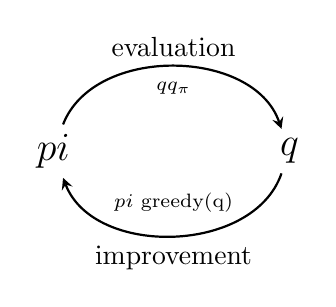
\begin{tikzpicture}[>=stealth, node distance=1.5cm, on grid, auto,
    arrow/.style = {thick,-stealth}]

    % States
    \node [] (center) {};
    \node [] (policy) [left=of center ] {\Large \(\gls{pi}\)};
    \node [] (values) [right=of center] {\Large \(\Gls{q}\)};

    % Transitions
    \draw [arrow] (policy) edge[bend left=70] node(E) {evaluation} (values);
    \draw [arrow] (values) edge[bend left=70] node(I) {improvement} (policy);
    \node [] () [below=15pt of E] {\scriptsize\(\Gls{q}\rightsquigarrow q_\pi\)};
    \node [] () [above=20pt of I] {\scriptsize\(\gls{pi}\rightsquigarrow\) 
        greedy(\Gls{q})};
\end{tikzpicture}
%     }
%     \captionsetup{margin=1.2em}
%     \caption{Generalized Policy Iteration.}
%     \label{fig:gpi_cycle}
% \end{wrapfigure}
% %
% In either method, the policy and action values are updated iteratively.
% Sutton and Barto~\cite{sutton2018} provide a graphic intuition for this 
% iterative cycle, which we have replicated in~\cref{fig:gpi_cycle}.

% A key distinction between Monte Carlo in this context and methods described 
% later is that Monte Carlo methods execute an entire episode. In the following 
% section, this principle will be applied to smaller segments of experience. 
% Additionally, we will reference \gls{mcts}, 
% a heuristic that simulates the results of future actions. Despite its name, 
% \gls{mcts} is distinct from the Monte Carlo methods discussed here.

%------------------------------------------------------------------------------
\section{Multi-Agent Reinforcement Learning}
\label{sec:marl-fundamentals}
%------------------------------------------------------------------------------

While single-agent \gls{rl} provides the foundational tools for sequential 
decision-making under uncertainty, many real-world problems involve 
multiple interacting agents whose decisions jointly determine outcomes. 
\Gls{marl} extends the single-agent framework to accommodate these multi-agent settings, 
introducing new challenges related to non-stationarity, coordination, and scalability. 
This section formalizes the \gls{marl} problem, introduces the dominant training paradigms, 
and surveys the key algorithmic approaches that underpin the contributions of this dissertation.

% \subsection{Problem Formalization}
% \label{subsec:marl-formalization}

% The transition from single-agent to multi-agent settings requires 
% extending the \gls{mdp} framework to account for multiple decision-makers 
% whose actions jointly influence state transitions and rewards. 
% Two primary formalisms capture this extension: \glspl{posg} and \glspl{dec-pomdp}.

% \subsubsection{Partially Observable Stochastic Games}

% A \gls{posg} generalizes the Markov game framework introduced 
% by \cite{littman1994} to settings with partial observability. 
% Formally, a \gls{posg} is defined by the tuple 
% $\langle \mathcal{I}, \mathcal{S}, \{\mathcal{A}_i\}_{i \in \mathcal{I}}, 
% \{\mathcal{O}_i\}_{i \in \mathcal{I}}, P, \{R_i\}_{i \in \mathcal{I}}, 
% \{Z_i\}_{i \in \mathcal{I}}, \gamma \rangle$, where $\mathcal{I} = \{1, \ldots, n\}$ 
% denotes the set of $n$ agents, $\mathcal{S}$ is the global state space, 
% $\mathcal{A}_i$ and $\mathcal{O}_i$ are the action and observation spaces 
% for agent $i$ respectively, 
% $P: \mathcal{S} \times \mathcal{A} \times \mathcal{S} \rightarrow [0,1]$ 
% defines the state transition probabilities conditioned on the joint action 
% $\mathbf{a} = (a_1, \ldots, a_n) \in \mathcal{A} = \prod_{i \in \mathcal{I}} 
% \mathcal{A}_i$, $R_i: \mathcal{S} \times \mathcal{A} \times \mathcal{S} \rightarrow \mathbb{R}$ 
% specifies the reward function for agent 
% $i$, $Z_i: \mathcal{S} \times \mathcal{A} \times \mathcal{O}_i \rightarrow [0,1]$ 
% defines the observation function for agent $i$, and $\gamma \in [0,1)$ 
% is the discount factor.

% This formalism captures the fundamental challenge of \gls{marl}: 
% from any individual agent's perspective, the environment appears 
% non-stationary because state transitions depend on the actions of other 
% agents whose policies may be simultaneously evolving \cite{busoniu2008}. 
% This non-stationarity violates the Markov property that guarantees convergence 
% in single-agent settings, making multi-agent learning substantially more challenging.

% \subsubsection{Decentralized Partially Observable Markov Decision Processes}

% The \gls{dec-pomdp} represents a special case of the \gls{posg} where all 
% agents share a common reward function: 
% \(\Gls{r}_1 = \Gls{r}_2 = \cdots = \Gls{r}_n = \Gls{r}\). 
% This shared reward structure makes the \gls{dec-pomdp} the canonical 
% formalism for fully cooperative multi-agent problems \cite{busoniu2008}. 
% Despite the cooperative objective, \glspl{dec-pomdp} remain computationally 
% challenging solving them optimally is NEXP-complete in the number of agents, 
% motivating the development of approximate solution methods \cite{busoniu2008}.

% In a \gls{dec-pomdp}, each agent $i$ maintains a policy 
% $\pi_i: \mathcal{O}_i \rightarrow \Delta(\mathcal{A}_i)$ 
% that maps local observations to action distributions. 
% The joint policy $\boldsymbol{\pi} = (\pi_1, \ldots, \pi_n)$ 
% induces a probability distribution over trajectories, 
% and the objective is to maximize the expected discounted return:
% \begin{equation}
%     J(\boldsymbol{\pi}) = \mathbb{E}\left[\sum_{t=0}^{\infty} \gamma^t R(s_t, \mathbf{a}_t, s_{t+1}) \mid \boldsymbol{\pi}\right]
%     \label{eq:joint-objective}
% \end{equation}

% \subsubsection{Joint Action Spaces and Scalability}

% A defining characteristic of multi-agent systems is the exponential growth of the joint action space. For $n$ agents each with $|\mathcal{A}_i| = k$ actions, the joint action space has cardinality $k^n$. This combinatorial explosion poses severe scalability challenges: naive approaches that enumerate joint actions become intractable even for moderate team sizes. The joint observation space $\mathcal{O} = \prod_{i \in \mathcal{I}} \mathcal{O}_i$ exhibits similar exponential scaling, compounding the difficulty of learning effective joint policies.

% \subsubsection{Cooperative, Competitive, and Mixed Settings}

% Multi-agent environments span a spectrum of agent relationships. 
% In \textit{cooperative} settings (as in \glspl{dec-pomdp}), agents 
% share a common objective and must coordinate to maximize collective reward. 
% \textit{Competitive} or zero-sum games represent the opposite extreme, 
% where one agent's gain is another's loss---exemplified by two-player 
% board games that motivated early game-theoretic \gls{rl} \cite{littman1994}. \textit{Mixed-motive} environments involve elements of both cooperation and competition, requiring agents to balance individual and collective interests.

% \cite{shoham2007} argue that clearly specifying the multi-agent 
% learning objective is essential for meaningful algorithm development and evaluation. 
% In cooperative settings, the objective is typically the shared reward signal of 
% Equation~\ref{eq:joint-objective}. For competitive settings, solution concepts from game 
% theory---such as \gls{nash}---provide alternative optimization targets, though computing 
% Nash equilibria in general-sum games is computationally intractable. This dissertation focuses 
% primarily on cooperative settings where the research questions center on training efficiency 
% rather than strategic equilibrium computation.


\subsection{Centralized Training with Decentralized Execution}
\label{subsec:ctde}

The \gls{ctde} paradigm has emerged as the dominant framework for cooperative \gls{marl}, 
elegantly resolving the tension between the coordination requirements of multi-agent 
learning and the decentralized execution constraints of real-world deployment 
\cite{lowe2020, foerster2018}.

\subsubsection{The Paradigm Explained}

Under \gls{ctde}, agents have access to additional information during training;
including global state, other agents' observations, and joint actions;
that is unavailable during execution. At deployment time, 
each agent acts based solely on its local observation, 
but the training process leverages centralized information to 
facilitate coordination learning. This paradigm is particularly well-suited 
to simulation-based training of robotic systems, 
where full observability can be assumed during training while physical 
sensor limitations constrain deployed agents.

The key insight of \gls{ctde} is that training and execution need not 
impose identical information constraints. By relaxing training-time observability, 
algorithms can address the credit assignment problem more effectively and 
stabilize learning in the face of multi-agent non-stationarity.

\subsubsection{Critic Architectures and Centralized Information}

The actor-critic architecture provides a natural implementation of \gls{ctde}: 
actors (policies) condition only on local observations to ensure decentralized 
executability, while critics (value functions) access centralized information 
to reduce variance and improve credit assignment. 
\cite{lowe2020} introduced \gls{maddpg}, which trains a 
centralized critic \(\Gls{q}_{\gls{i}}(\gls{s}, \gls{a}_1, \ldots, \gls{a}_n)\) 
for each agent that conditions on the global state and all agents' actions. 
This centralized critic provides stable gradient estimates while 
maintaining decentralized policies.

% \begin{wrapfigure}[10]{R}{0.4\textwidth}
%     \vspace*{-1em}
%     % \vspace*{-2em}
%     \centering
%     \documentclass{standalone}
\usepackage[dvipsnames]{xcolor}
\usepackage{tikz}
\usetikzlibrary{positioning, shapes, arrows,}

\begin{document}
\colorlet{DarkGreen}{Black!25!Green}
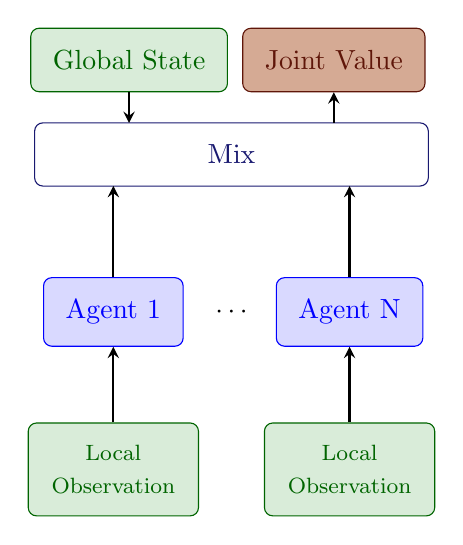
\begin{tikzpicture}[>=stealth, node distance=2cm, on grid, auto,
    entry/.style = {draw, rectangle, inner sep=8pt, rounded corners=3pt,
                    minimum width=1.5cm},
    greenEntry/.style = {draw, rectangle, inner sep=8pt, rounded corners=3pt,
                minimum width=1.5cm, align=center, DarkGreen, fill=Green!15},
    blueEntry/.style = {draw, rectangle, inner sep=8pt, rounded corners=3pt,
                    minimum width=1.5cm, Blue, fill=Blue!15},
    arrow/.style = {thick,-stealth}]

    % Entries
    \node [] (center) {\(\cdots\)};
    \node [blueEntry] (agent_1) [left =1.5cm of center] {Agent 1\ };
    \node [blueEntry] (agent_n) [right=1.5cm of center] {Agent N};
    \node [entry, MidnightBlue] (mix) [above=of center, minimum width=5cm] {Mix};
    \node [greenEntry] (state) [above left=1.2cm and 1.3cm of mix] 
        {Global State};
    \node [entry, Sepia, fill=Sepia!25] (value) [above right=1.2cm and 1.3cm of mix] {Joint Value};
    \node [greenEntry, text width=1.6cm] (obs_1) [below=of agent_1] 
        {\footnotesize Local Observation};
    \node [greenEntry, text width=1.6cm] (obs_n) [below=of agent_n] 
        {\footnotesize Local Observation};

    % Relations
    \draw [arrow] (obs_1) -- (agent_1);
    \draw [arrow] (obs_n) -- (agent_n);
    \draw [arrow] (agent_1) -- +(0,1.6);
    \draw [arrow] (agent_n) -- +(0,1.6);
    \draw [arrow] (state) -- +(0,-0.8);
    \draw [arrow] (value)+(0,-0.8) -- (value) ;
\end{tikzpicture}


\end{document}
%     \caption{Basic \gls{ctde}.}
%     \label{fig:basic_ctde}
% \end{wrapfigure}
%
\begin{figure}[!ht]
    \centering
    \documentclass{standalone}
\usepackage[dvipsnames]{xcolor}
\usepackage{tikz}
\usetikzlibrary{positioning, shapes, arrows,}

\begin{document}
\colorlet{DarkGreen}{Black!25!Green}
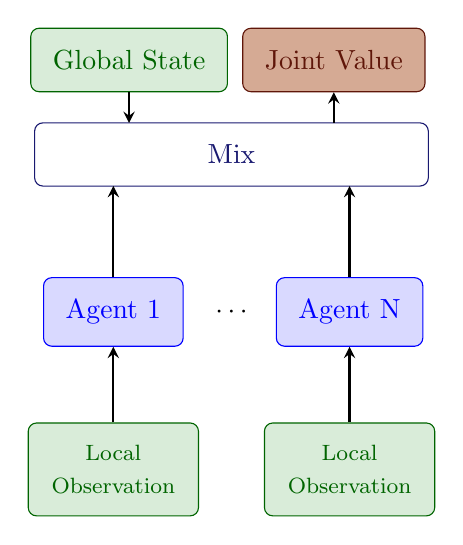
\begin{tikzpicture}[>=stealth, node distance=2cm, on grid, auto,
    entry/.style = {draw, rectangle, inner sep=8pt, rounded corners=3pt,
                    minimum width=1.5cm},
    greenEntry/.style = {draw, rectangle, inner sep=8pt, rounded corners=3pt,
                minimum width=1.5cm, align=center, DarkGreen, fill=Green!15},
    blueEntry/.style = {draw, rectangle, inner sep=8pt, rounded corners=3pt,
                    minimum width=1.5cm, Blue, fill=Blue!15},
    arrow/.style = {thick,-stealth}]

    % Entries
    \node [] (center) {\(\cdots\)};
    \node [blueEntry] (agent_1) [left =1.5cm of center] {Agent 1\ };
    \node [blueEntry] (agent_n) [right=1.5cm of center] {Agent N};
    \node [entry, MidnightBlue] (mix) [above=of center, minimum width=5cm] {Mix};
    \node [greenEntry] (state) [above left=1.2cm and 1.3cm of mix] 
        {Global State};
    \node [entry, Sepia, fill=Sepia!25] (value) [above right=1.2cm and 1.3cm of mix] {Joint Value};
    \node [greenEntry, text width=1.6cm] (obs_1) [below=of agent_1] 
        {\footnotesize Local Observation};
    \node [greenEntry, text width=1.6cm] (obs_n) [below=of agent_n] 
        {\footnotesize Local Observation};

    % Relations
    \draw [arrow] (obs_1) -- (agent_1);
    \draw [arrow] (obs_n) -- (agent_n);
    \draw [arrow] (agent_1) -- +(0,1.6);
    \draw [arrow] (agent_n) -- +(0,1.6);
    \draw [arrow] (state) -- +(0,-0.8);
    \draw [arrow] (value)+(0,-0.8) -- (value) ;
\end{tikzpicture}


\end{document}
    \caption{Basic CTDE.}
    \label{fig:basic_ctde}
\end{figure}

\Cref{fig:basic_ctde} shows an example of this in which centralization is
performed by a \emph{mixing} function that combines a global state with 
the actions of each agent to provide a single state or action-state value.

\cite{foerster2018} extended this approach with \gls{coma}, 
which uses a centralized critic to compute counterfactual baselines. 
By comparing an agent's action against the expected value of 
marginalizing over that agent's action distribution, 
\gls{coma} isolates each agent's contribution to the team reward, 
directly addressing the credit assignment problem in cooperative settings.

Value decomposition methods offer an alternative \gls{ctde} implementation. 
QMIX \cite{rashid2018} learns individual utility functions 
\(\Gls{q}_{\gls{i}}(\gls{o}_{\gls{i}}, \gls{a}_{\gls{i}})\)
that are combined through a monotonic mixing network to 
approximate the joint action-value function.
This factorization enables decentralized execution while 
maintaining consistency with a centralized training objective. 
The monotonicity constraint ensures that greedy action 
selection with respect to individual utilities yields 
globally optimal joint actions.

\subsubsection{Benefits and Limitations}

\gls{ctde} offers several advantages for cooperative \gls{marl}.
By conditioning critics on global information, the paradigm reduces 
non-stationarity from individual agents' perspectives and enables 
more effective credit assignment. The centralized training phase can exploit 
simulation environments where full observability is computationally free, 
while the decentralized execution phase respects real-world communication constraints.

However, \cite{zhou2023} question whether \gls{ctde} is universally necessary, 
demonstrating that simpler approaches can match or exceed \gls{ctde} 
methods in certain domains. Their analysis suggests that the benefits 
of centralized training depend on task characteristics, 
particularly the degree of coordination required and the 
informativeness of global state beyond local observations. 
Despite these caveats, \gls{ctde} remains the predominant 
paradigm for cooperative \gls{marl}, and all contributions 
in this dissertation operate within the \gls{ctde} framework.

\subsection{Independent Learning versus Centralized Methods}
\label{subsec:independent-vs-centralized}

A fundamental design choice in \gls{marl} is whether agents should 
learn independently, treating other agents as part of the environment, 
or jointly, explicitly modeling multi-agent interactions.

\subsubsection{Independent Learning and IPPO}

\Gls{ippo} represents the simplest multi-agent extension of policy gradient methods: 
each agent independently optimizes its policy using the standard \gls{ppo} objective, 
treating other agents as non-stationary environmental dynamics. 
Despite this seeming naivety, \cite{witt2020} demonstrated that independent 
learning performs surprisingly well in many cooperative settings, challenging the 
assumption that explicit multi-agent coordination mechanisms are essential.

\cite{yu2022} provided a systematic investigation of \gls{mappo}'s effectiveness, 
finding that with careful implementation choices (proper input normalization, 
value function clipping, and appropriate network architectures)
independent and shared-parameter variants of \gls{ppo} achieve 
state-of-the-art performance across diverse cooperative benchmarks. 
Their work emphasized that implementation details often matter 
more than algorithmic innovations, establishing \gls{mappo} 
as a strong baseline for cooperative \gls{marl}.

The success of independent learning methods may be attributed to several factors. 
First, modern policy optimization algorithms like \gls{ppo} are relatively robust 
to non-stationarity due to their conservative update mechanisms. Second, 
in cooperative settings where agents share objectives, the gradient directions 
of independently learning agents may naturally align, reducing interference. 
Third, shared reward signals provide implicit coordination even without 
explicit communication.

% \subsubsection{Value Decomposition Approaches}

% Value decomposition methods address the credit assignment problem 
% by factoring the joint value function into agent-specific contributions. 
% \Gls{vdn} assumes additive decomposition: 
% \(\Gls{q} = \sum_{i\in\Gls{i}} \Gls{q}_{\gls{i}}\). 
% QMIX relaxes this to monotonic combinations, 
% learning a mixing network that satisfies $\frac{\partial Q_{tot}}{\partial Q_i} \geq 0$. 
% QTRAN removes monotonicity constraints entirely, 
% enabling representation of arbitrary factorizable 
% value functions at the cost of more complex optimization.

% These methods offer an alternative to policy gradient approaches for discrete action spaces, 
% particularly in settings where off-policy learning from replay buffers is desirable. 
% However, the monotonicity constraints of VDN and QMIX limit representational expressiveness, 
% and non-monotonic methods like QTRAN face optimization challenges in practice.

\subsubsection{Communication Learning}

An orthogonal approach to multi-agent coordination involves learning to communicate. 
\cite{sukhbaatar2016} introduced CommNet, where agents pass continuous messages 
that are averaged and concatenated with local observations. 
Subsequent work has explored attention-based communication, 
graph-structured message passing, and learned communication protocols.

Communication learning is particularly relevant when local 
observations are insufficient for effective decision-making 
and agents benefit from sharing information. 
However, learned communication adds architectural complexity 
and can be difficult to interpret. For many cooperative tasks, 
the implicit coordination enabled by shared training or 
centralized critics provides sufficient coordination without
explicit communication.

\subsection{Multi-Agent PPO Variants}
\label{subsec:mappo-variants}

\Gls{ppo} has become the algorithm of choice for many \gls{marl} 
applications due to its stability, sample efficiency, 
and ease of implementation. Several multi-agent variants extend 
\gls{ppo} to address specific challenges in cooperative settings.

\subsubsection{MAPPO and Parameter Sharing}

\Gls{mappo} applies \gls{ppo} to multi-agent settings, 
optionally with parameter sharing across agents. 
In the fully shared variant, a single policy network 
parameterizes all agents' behaviors, with agent 
identity encoded through observation augmentation. 
\cite{yu2022} demonstrated that \gls{mappo} with 
shared parameters achieves strong performance across 
diverse benchmarks while dramatically reducing the 
number of trainable parameters.

Parameter sharing offers several advantages beyond reduced memory footprint. 
By aggregating experiences from all agents, shared policies enjoy improved 
sample efficiency. Shared representations can capture agent-invariant 
skills that transfer across roles. 
However, full parameter sharing assumes that a single policy can 
adequately represent all agents' behaviors;
an assumption that breaks down in settings with intrinsic heterogeneity, 
as explored in subsequent chapters.

\subsubsection{HAPPO}

\Gls{happo}, introduced by \cite{zhong2024}, addresses the challenge of 
heterogeneous agents with different observation and action spaces. 
The key insight is that the standard multi-agent policy gradient 
objective decomposes across agents when updates are performed 
sequentially with appropriate advantage computation. 
\gls{happo} maintains separate policy networks for each agent type while 
ensuring monotonic improvement guarantees analogous to those provided by 
\gls{trpo} and \gls{ppo} in single-agent settings.

The \gls{happo} update rule factorizes the joint policy gradient into 
sequential single-agent updates:
\begin{equation}
    \nabla_{\theta_{i}} \boldsymbol{\pi}
    = \gls{expRet}_{\boldsymbol{\pi}}\left[
        \sum_{a_1, \ldots, a_{i-1}} \prod_{j<i} \gls{pi}_j(\gls{a}_j | \gls{o}_j) 
        \cdot \nabla_{\theta_{i}} 
        \log \gls{pi}_{\gls{i}}(\gls{a}_{\gls{i}} | \gls{o}_{\gls{i}}) 
        \cdot \hat{\gls{adv}}_{\gls{i}}(\gls{s}, \gls{a}_1, \ldots, \gls{a}_{\gls{i}})
    \right]
\end{equation}
where \(\hat{\gls{adv}}_{\gls{i}}\) is the multi-agent advantage for the 
\(gls{i}\)-th agent, accounting for the actions of preceding agents. 
This sequential decomposition enables theoretically-grounded policy 
updates without requiring the restrictive assumptions of parameter sharing.

\subsubsection{Trust Region Methods in Multi-Agent Settings}

Trust region methods constrain policy updates to prevent large, 
destabilizing changes. \gls{trpo} enforces a \gls{kl} divergence 
constraint between successive policies, while \gls{ppo} 
approximates this constraint through clipped surrogate objectives. 
In multi-agent settings, maintaining trust region properties becomes more 
complex because the joint policy space is the product of individual policy spaces.

\cite{li2023c} extends trust region optimization to multi-agent 
settings through \gls{matrpo}, providing theoretical guarantees for 
joint policy improvement while maintaining computational tractability. 
The heterogeneous variants (\gls{hatrpo}, \gls{happo}) extend 
these guarantees to settings where agents may have different 
policy parameterizations \cite{zhong2024}.

% #TODO: Refer to Contribution X or as "Chapter-X"?
These multi-agent \gls{ppo} variants form the algorithmic foundation 
for the contributions of this dissertation. 
Contribution~1 employs \gls{ppo} within a curriculum learning framework, 
Contribution~2 extends parameter sharing to heterogeneous settings 
through implicit indication, and 
Contribution~3 compares architectural versus representational 
approaches to heterogeneity using \gls{mappo} and \gls{happo} 
as baseline implementations. The choice of \gls{ppo}-based methods 
is motivated by their empirical effectiveness, implementation stability, 
and widespread adoption in the \gls{marl} community.

%------------------------------------------------------------------------------
\section{Scalability Challenges in MARL}
\label{sec:scalability-challenges}
%------------------------------------------------------------------------------

The transition from single-agent to multi-agent reinforcement 
learning introduces fundamental scalability challenges that 
constrain the practical applicability of \gls{marl} algorithms. 
As team sizes grow, computational costs escalate rapidly, 
sample efficiency degrades, and the coordination problem 
becomes increasingly intractable. 
This section examines the sources of these scalability bottlenecks, 
surveys approaches for mitigating them through parameter sharing, 
and characterizes the benchmark environments used to evaluate scalability. 
These challenges directly motivate the contributions of this dissertation: 
% #TODO: Contribution X ref?
Contribution~1 addresses training cost through curriculum-based team scaling, 
Contribution~2 extends parameter sharing to heterogeneous settings through 
implicit indication, and 
Contribution~3 compares paradigms for handling heterogeneity at scale.

\subsection{Computational Complexity and Team Size}
\label{subsec:computational-complexity}

The exponential scaling of joint spaces with respect to the 
number of agents represents the most fundamental barrier to 
scaling \gls{marl} \cite{gronauer2022, zhang2021}. 
Understanding the sources and implications of this complexity 
is essential for developing efficient training strategies.

\subsubsection{Exponential Growth of Joint Spaces}

Consider a multi-agent system with \(n\in\gls{naturals}\) agents, 
where each agent \(\gls{i}\) has observation space \(\Gls{o}_{\gls{i}}\)
with \(|\Gls{o}_{\gls{i}}| = d_{\gls{o}}\) dimensions and action space 
\(\Gls{A}_{\gls{i}}\) with \(|\Gls{A}_{\gls{i}}| = k\) discrete actions. 
The joint observation space \(\Gls{o} = \prod_{i=1}^{n} \Gls{o}_i\)
grows as (Big \(O\)) \(\mathcal{O}(d_o^n)\), while the joint action space 
\(\Gls{a} = \prod_{i=1}^{n} \Gls{a}_{i}\) grows as \(\mathcal{O}(k^n)\). 
This combinatorial explosion means that algorithms which explicitly 
represent joint spaces become intractable even for moderate team sizes 
\cite{hernandez-leal2019}.

For policy gradient methods, the challenge manifests differently but remains severe. 
The number of parameters required to represent \(n\) separate policies scales linearly 
as \(\mathcal{O}(n \cdot p)\), where \(p\) is the parameter count per policy. 
However, the effective sample complexity scales super-linearly because each 
agent's learning signal is corrupted by the non-stationarity induced by 
other agents' simultaneous policy updates \cite{zhang2021}. 
Empirically, training time often exhibits polynomial or even exponential 
dependence on team size, depending on the degree of coordination required.

\subsubsection{Training Time and Sample Efficiency}

The relationship between team size and training cost is multifaceted. 
First, each environment step generates experience for all \(n\) agents, 
suggesting that per-agent sample efficiency might improve with larger teams. 
However, this apparent benefit is offset by several factors. 
The credit assignment problem becomes increasingly difficult as the 
number of contributing agents grows \cite{foerster2018}. 
Variance in gradient estimates increases with team size because 
each agent's gradient depends on the actions of all other agents. 
Exploration becomes more challenging as the probability that all 
agents simultaneously discover beneficial joint behaviors decreases 
exponentially \cite{hernandez-leal2019}.

\cite{liu2024a} provide a systematic investigation of scaling behavior 
in cooperative \gls{marl}, demonstrating that na\"ive scaling leads 
to sublinear performance improvements despite linear increases in 
computational resources. Their analysis reveals that coordination overhead
(the additional learning required for agents to align their behaviors)
dominates training cost in tightly-coupled tasks. 
These findings underscore the need for training strategies that can 
amortize coordination learning across team configurations, 
a gap that Contribution~1 addresses through curriculum-based approaches.

\subsubsection{Implications for Practical Deployment}

The scalability challenge has direct implications for real-world applications. 
Autonomous drone swarms, robotic warehouse systems, and distributed sensor networks 
often involve tens to hundreds of agents operating under tight latency constraints. 
Training policies for these systems using na\"ive \gls{marl} algorithms would require 
computational resources that scale prohibitively with fleet size.

Consider a target deployment of \(n_{\text{target}} = 100\) agents. 
Training separate policies requires optimizing \(100 \cdot p\) parameters, 
collecting sufficient samples for each policy to converge, and managing 
the non-stationarity induced by 99 simultaneously adapting teammates. 
Even with parallelization across environment instances, the coordination 
learning overhead makes direct training at target scale computationally expensive. 
This motivates the core question of Contribution~1: can training smaller teams 
and transferring policies to larger configurations reduce total training cost 
while preserving final performance?

\subsubsection{Normalized Metrics: Agent-Steps}

Comparing training efficiency across different team sizes requires 
careful consideration of cost metrics. Wall-clock time depends on 
hardware and implementation details. Raw environment steps disadvantage 
larger teams that generate more per-step experience. 
To enable fair comparison, this dissertation adopts the \textit{agent-steps} metric, 
defined as the product of the number of agents and the number of environment steps:
\begin{equation}
    \text{Agent-Steps} = n \times \Gls{t}
    \label{eq:agent-steps}
\end{equation}
where \(n\) is the number of agents and \(\Gls{t}\) is the number of environment steps. 
This metric normalizes for team size by accounting for the total experience collected, 
providing a basis for comparing curriculum strategies that train at different 
scales before converging to a target configuration.

The agent-steps metric directly connects to sample efficiency: 
lower agent-steps to achieve a given performance level indicates 
more efficient use of collected experience. Contribution~1 uses 
this metric to evaluate whether pretraining with smaller teams can 
reduce total agent-steps while maintaining or improving final performance.

\subsection{Parameter Sharing for Efficiency}
\label{subsec:parameter-sharing}

Parameter sharing offers a direct approach to mitigating the scalability 
challenges of \gls{marl}: instead of maintaining $n$ separate policy networks, 
agents share some or all parameters, reducing memory footprint, improving 
sample efficiency, and enabling generalization across agents \cite{terry2020}. 
However, parameter sharing introduces its own challenges, particularly when 
agents require differentiated behaviors.

\subsubsection{Full Parameter Sharing}

In the fully shared paradigm, a single policy network \(\gls{pi}_\theta\) 
parameterizes all agents' behaviors. Agents are distinguished through 
observation augmentation, typically by appending a one-hot encoding 
of agent identity to the observation vector. This approach reduces 
the number of trainable parameters from \(\mathcal{O}(n \cdot p)\) 
to \(\mathcal{O}(p)\), a dramatic reduction for large teams.

Full parameter sharing assumes that agents are sufficiently similar 
that a single policy can adequately represent all required behaviors. 
This assumption holds in many cooperative settings with homogeneous agents, 
where the optimal behavior in a given state-action context is agent-invariant. 
\cite{yu2022} demonstrated that \gls{mappo} with full parameter sharing 
achieves state-of-the-art performance across diverse cooperative benchmarks, 
establishing shared policies as a strong default approach.

Beyond memory efficiency, full parameter sharing improves 
sample efficiency by pooling experience across agents. 
Each environment step contributes \(n\) training samples to a 
single policy, effectively multiplying the data available for learning. 
This pooling also enables implicit coordination: because all agents 
optimize the same objective with the same parameters, their learned 
behaviors naturally align without explicit communication mechanisms.

\subsubsection{Limitations of Full Sharing}

Despite these advantages, full parameter sharing fails when agents 
require fundamentally different behaviors. 
Three categories of differentiation challenge the shared policy assumption:

\textit{Behavioral heterogeneity} 
arises when agents occupy different roles despite sharing the same capabilities. 
In predator-prey scenarios, some agents may specialize as chasers while others 
serve as blockers. A shared policy with one-hot agent identifiers can, in principle, 
learn role-specific behaviors, but this places the burden of role differentiation 
entirely on the policy network's capacity to condition on the agent index.

\textit{Observation heterogeneity} 
occurs when agents have access to different sensory information. 
A drone equipped with a camera and another with \glsentryshort{lidar} receive 
observations from incompatible spaces, precluding direct parameter sharing. 
Similarly, agents at different positions in spatially-structured tasks
(such as the lead, middle, and rear walkers in Multiwalker)
receive observations with different semantic content.

\textit{Action heterogeneity} 
manifests when agents have different available actions. 
A ground robot and an aerial vehicle share the goal of 
reaching a target but command distinct actuator spaces. 
A shared policy cannot directly output actions for both 
agent types without architectural modifications.

These limitations motivate the development of selective and 
heterogeneous parameter sharing approaches that preserve 
efficiency benefits while accommodating agent differences.

\subsubsection{Selective Parameter Sharing}

\cite{christianos2021} introduced selective parameter sharing as a 
middle ground between full sharing and fully independent policies. 
Their approach groups agents based on similarity criteria, which may 
be predefined or learned,and shares parameters only within groups. 
This enables differentiation between agent types while maintaining 
sharing benefits within each type.

The grouping mechanism can be implemented in various ways. 
Explicit grouping assigns agents to predefined types based on domain 
knowledge (e.g., agent position, sensor suite, or capability set). 
Learned grouping discovers agent clusters during training, 
potentially adapting as policies specialize. 
Hierarchical architectures share early layers that extract common 
features while maintaining type-specific heads for final action selection.

Selective parameter sharing reduces parameters from \(\mathcal{O}(n \cdot p)\) 
to \(\mathcal{O}(k \cdot p)\), where \(k\) is the number of agent groups. 
This scaling is advantageous when \(k \ll n\), as is typical in many applications 
where a small number of distinct agent types operate in larger numbers. 
However, the approach requires specification of the grouping structure, 
which may not be obvious a priori and may not align with the natural 
structure of learned behaviors.

\subsubsection{Agent Indication and Identification}

For shared policies to differentiate agent behaviors, 
they require some form of agent indication; a signal that 
identifies which agent is currently executing the policy \cite{terry2020}. 
The choice of indication mechanism has significant implications for 
learning dynamics and generalization.
One-hot encoding, Learned embeddings, and Positional encoding
are indication methods further discussed in \cref{subsec:agent-indication}.

These explicit indication methods share a common limitation: 
they require agents to occupy compatible observation and action spaces. 
When agents differ structurally, explicit indication cannot resolve the 
dimensional mismatch between agent types. This limitation motivates the 
implicit indication approach developed in Contribution~2, 
where agent identity is inferred from the pattern of populated elements 
in a homogenized observation space rather than from explicit identifiers.

\subsubsection{Trade-offs: Efficiency versus Specialization}

Parameter sharing introduces a fundamental trade-off between 
computational efficiency and behavioral specialization. 
Full sharing maximizes efficiency but limits expressiveness. Separate 
policies maximize expressiveness but sacrifice efficiency and generalization. 
The optimal point on this spectrum depends on task characteristics: 
homogeneous tasks favor sharing, while heterogeneous tasks require differentiation.

\cite{hao2022} investigate this trade-off through adaptive agent 
grouping mechanisms that adjust sharing structure during training. 
Their approach begins with full sharing and progressively partitions 
agents into specialized groups as behavioral divergence emerges. 
This adaptive strategy attempts to achieve the best of both worlds, 
maintaining sharing when possible while allowing differentiation when necessary.

The parameter sharing literature largely assumes that agents occupy compatible spaces;
that sharing is possible, and the question is merely how much to share. 
Contribution~2 extends this literature by developing a sharing mechanism 
for agents with incompatible observation spaces through observation homogenization,
while Contribution~3 compares this representational approach against architectural 
solutions that encode heterogeneity through specialized network structures.


%------------------------------------------------------------------------------
\subsection{Benchmark Environments and Evaluation}
\label{subsec:benchmark-environments}
%------------------------------------------------------------------------------

The development and evaluation of scalable \gls{marl} algorithms requires 
benchmark environments that exhibit relevant coordination challenges, 
support variable team sizes, and enable controlled experimentation. 
This subsection surveys the evolution of \gls{marl} benchmarks and 
characterizes the specific environments used in this dissertation.

\subsubsection{Evolution of MARL Benchmarks}

% #TODO: Clean up this lead-in to benchmarks
% Early \gls{marl} research relied on simple matrix games and 
% small-scale simulations that, while theoretically informative, 
% failed to capture the complexity of realistic multi-agent coordination. 
% The success of deep \gls{rl} on single-agent benchmarks like Atari 
% motivated the development of more challenging multi-agent environments.

% The StarCraft Multi-Agent Challenge (SMAC) \cite{samvelyan2019} 
% established a widely-adopted benchmark based on micromanagement 
% scenarios from the real-time strategy game StarCraft II. 
% SMAC's popularity stems from its diversity of scenarios, 
% clear evaluation metrics, and challenging coordination requirements. 
% However, \cite{ellis2023} identified limitations in SMAC's original scenarios, 
% including exploitable opponent behaviors and insufficient scenario diversity, 
% motivating the development of SMACv2 with procedurally generated maps 
% and more robust evaluation protocols.

% \Gls{grf} \cite{kurach2020} provides another influential benchmark based on simulated football. 
% The environment supports variable team sizes and requires both local coordination 
% (passing, positioning) and global strategy (formations, set pieces). 
% However, its computational cost limits its accessibility for resource-constrained research.

PettingZoo \cite{terry2021} standardized the multi-agent environment 
interface through a Gymnasium-compatible API, enabling systematic 
benchmarking across diverse domains. 
The standardization facilitated the development of environment 
suites like the \gls{sisl} environments and Level-Based Foraging, 
which are used in this dissertation.

Recent work has emphasized JAX-based implementations for accelerated training. 
JaxMARL \cite{rutherford2023} provides GPU-accelerated versions of popular benchmarks,
enabling training speeds orders of magnitude faster than CPU-based alternatives. 
This acceleration is particularly valuable for scalability research, 
where the goal is often to reduce training cost; 
a goal that faster simulators directly support.

\subsubsection{Environments Used in This Dissertation}

The contributions of this dissertation employ environments 
selected to span a range of coordination challenges, 
heterogeneity types, and scalability characteristics.

\textit{Waterworld} \cite{gupta2017}, from the \gls{sisl} suite, 
presents a continuous-space coordination task where agents must 
collectively capture food targets while avoiding poison. 
Agents observe their surroundings through egocentric, range-limited 
sensors and control their movement through continuous thrust actions. 
All agents share identical observation and action spaces, 
making Waterworld a testbed for pure parameter sharing approaches. 
The environment supports arbitrary team sizes, enabling curriculum 
learning experiments that train at small scales and transfer to larger teams. 
Coordination requirements are relatively modest: agents benefit from distributing 
across the environment but do not require tight temporal synchronization. 
This makes Waterworld well-suited for evaluating whether curriculum-based 
scaling provides benefits even when coordination overhead is limited.

\textit{Multiwalker} \cite{gupta2017}, also from the \gls{sisl} suite, 
presents a physically-coupled coordination challenge where bipedal robots 
must cooperatively transport a package across terrain. Unlike Waterworld, 
Multiwalker exhibits structural heterogeneity: agents at different 
positions (lead, middle, rear) receive observations with different 
semantic content and face different balance constraints. 
The task requires tight temporal coordination; if one agent stumbles, 
the entire team fails. This sensitivity to coordination errors makes 
Multiwalker a challenging testbed for scalability: larger teams 
introduce more potential failure points, potentially making small-team 
pretraining particularly valuable as a stabilizing mechanism. 
Multiwalker's fixed-position heterogeneity also motivates investigation 
of how observation differences interact with parameter sharing approaches.

\textit{Level-Based Foraging} (\gls{lbf}) \cite{papoudakis2021} provides 
a discrete grid-world environment with dynamic, intrinsic heterogeneity. 
Agents and food items are assigned skill levels, and food can only be 
collected when the combined levels of adjacent agents meet or exceed 
the food's requirement. This creates dynamic role dependencies: 
the optimal behavior for a given agent depends on both its own level 
and the composition of nearby teammates. \Gls{lbf}'s observation space 
scales with team size, as agents must observe the positions and levels 
of other agents, creating challenges for fixed-architecture policy transfer. 
The environment's discrete action space and clear coordination requirements 
make it a standard benchmark for cooperative \gls{marl}.

\subsubsection{Toward Domain-Specific Benchmarks}

While general-purpose benchmarks enable algorithm comparison across diverse settings, 
they may not capture the specific challenges of heterogeneous agent systems. 
Existing benchmarks either feature homogeneous agents (Waterworld, SMAC) 
or exhibit only limited forms of heterogeneity (positional differences 
in Multiwalker, level differences in \gls{lbf}).

To provide a controlled testbed for observation-space heterogeneity, 
Contributions~2 and~3 introduce \textit{HyperGrid}, a custom environment 
based on the MiniGrid framework \cite{chevalier-boisvert2023}. 
HyperGrid is an \(n\)-dimensional discrete grid environment where 
agents have configurable observation ``channels'' that determine 
which aspects of the environment they can perceive. 
This configurability enables systematic investigation of how 
observation heterogeneity affects learning, parameter sharing, 
and generalization.

HyperGrid addresses a particular gap in existing benchmarks: 
while Waterworld, Multiwalker, and \gls{lbf} enable evaluation 
of scalability and coordination, none provide fine-grained 
control over observation-space structure. 
The configurable heterogeneity of HyperGrid isolates the 
effects of observation differences from other confounding factors, 
enabling the controlled comparisons that underpin Contributions~2 and~3.

\subsubsection{Evaluation Metrics and Methodology}

Meaningful comparison of scalability approaches requires consistent evaluation methodology. 
This dissertation adopts several practices from the benchmarking literature.

\textit{Performance metrics} focus on cumulative episodic reward, 
normalized by episode length where appropriate to enable comparison 
across configurations with different time horizons. 
For curriculum learning experiments, final performance is evaluated 
at the target team size, while training efficiency is measured in agent-steps.

\textit{Statistical reliability} is ensured through multiple sample runs. 
The stochasticity of both environment dynamics and learning algorithms 
necessitates sufficient replication to distinguish genuine effects from noise.

\textit{Controlled comparison} requires matching hyperparameters and 
network architectures across methods wherever possible. 
When methods differ structurally (e.g., architectural versus 
representational approaches), comparison focuses on performance 
given equivalent computational budgets or parameter counts.

These evaluation practices inform the experimental designs of all 
three contributions, enabling fair comparison of curriculum strategies 
(Contribution~1), parameter sharing approaches (Contribution~2), 
and paradigms for handling heterogeneity (Contribution~3).

%------------------------------------------------------------------------------
\section{Heterogeneous Multi-Agent Reinforcement Learning}
\label{sec:heterogeneous-marl}
%------------------------------------------------------------------------------

The preceding sections have established the foundations of \gls{rl} and \gls{marl}, 
along with the scalability challenges that arise as team sizes grow. However, 
an additional dimension of complexity emerges when agents within a team are not identical. 
This section examines \gls{harl}, a subfield that addresses the unique challenges 
posed by teams of structurally or behaviorally distinct agents. 
Understanding heterogeneity is central to the contributions of this dissertation, 
as both the implicit indication framework (C2) and the architectural comparison study (C3) 
directly engage with the problem of training shared policies across non-identical agents.

\subsection{Taxonomy of Heterogeneity}
\label{subsec:taxonomy-heterogeneity}

The term ``heterogeneous'' in \gls{marl} encompasses multiple distinct 
phenomena that require different algorithmic treatments. 
This dissertation adopts a taxonomy that distinguishes between two primary forms 
of agent heterogeneity: behavioral heterogeneity and intrinsic heterogeneity.

\textbf{Behavioral heterogeneity} arises when agents share identical observation 
and action spaces but develop distinct policies through independent learning processes. 
In this setting, all agents perceive the environment through the same sensory 
modalities and can execute the same set of actions, yet they may specialize 
into different roles or strategies during training. For example, in a predator-prey 
scenario, multiple identical predator agents might naturally differentiate into 
flankers and chasers despite having equivalent capabilities \cite{calvo2018}. 
Behavioral heterogeneity emerges from the learning dynamics rather than from 
any structural differences between agents. This form of heterogeneity is often 
desirable, as role differentiation can improve team performance by reducing 
redundancy and enabling complementary behaviors \cite{wakilpoor2020}.

\textbf{Intrinsic heterogeneity}, in contrast, refers to fundamental 
structural differences in agents' interfaces with the environment. 
Agents may differ in their observation spaces (what they can perceive), 
their action spaces (what they can do), or both. The conditions in 
\cite{zhong2024} describe an intrinsically heterogeneous multi-agent 
system where there exists at least one pair of agents \((i, j)\)
such that \(\Gls{o}_i \neq \Gls{o}_j\) or \(\Gls{a}_i \neq \Gls{a}_j\), 
where \(\Gls{a}_{\gls{i}}\) and \(\Gls{a}_{\gls{i}}\) denote the 
observation and action spaces of agent \(\gls{i}\), respectively.

It should be noted that while Observation-space and 
Action-space differences are intuitive, intrinsic heterogeneity 
is not restricted to those features. For example, differences
in reward functions or transition state-transition probabilities.

The distinction between behavioral and intrinsic heterogeneity has significant 
implications for algorithm design. Behavioral heterogeneity can often be 
accommodated through parameter sharing approaches that allow identical 
network architectures to develop specialized behaviors through distinct 
parameter updates \cite{christianos2021}. Intrinsic heterogeneity, however, 
poses a more fundamental challenge: when agents have differently-dimensioned 
observation or action spaces, standard parameter sharing becomes impossible 
without additional mechanisms to reconcile these structural differences.

A useful conceptual framing considers the relationship between agent type 
and agent identity. In behaviorally heterogeneous systems, agents may be 
individually distinct (different identities) while belonging to the 
same type (same interface). In intrinsically heterogeneous systems, 
different agent types exist, and agents of different types have genuinely 
incompatible interfaces. This dissertation's contributions focus primarily 
on intrinsic heterogeneity, specifically observation-space heterogeneity, 
as this represents the more challenging and practically relevant case for 
real-world deployments where sensor diversity is common.

% #TODO: Add drone multi agent graphic from prospectus presentation.
The challenge of heterogeneity is compounded by the fact that many 
real-world multi-agent systems exhibit both forms simultaneously. 
A drone swarm might include quadcopters and fixed-wing aircraft 
(intrinsic heterogeneity in both observations and actions) that each 
develop specialized patrol behaviors (behavioral heterogeneity within type). 
Effective \gls{harl} algorithms must therefore provide mechanisms that can 
handle the full spectrum of heterogeneity while remaining computationally tractable.

\subsection{Agent Indication Methods}
\label{subsec:agent-indication}

When training shared policies across multiple agents, a fundamental 
question arises: how should agents be distinguished from one another? 
This question becomes particularly acute in heterogeneous settings, 
where the policy must produce appropriate behavior for agents with 
different capabilities. The literature has developed 
several approaches to \textbf{agent indication}; mechanisms that allow 
a shared policy to condition its behavior on agent identity or type.

The most straightforward approach is \textbf{one-hot encoding}, 
where each agent receives a binary vector appended to its 
observation that uniquely identifies it within the team. 
For a team of \(n\) agents, agent \(\gls{i}\) receives an 
indicator vector\(\mathbf{e}_i \in \{0,1\}^n\) with a single 
non-zero element at position \(\gls{i}\). 
This approach is simple to implement and has demonstrated 
promising performance in \cite{terry2020}. 
However, one-hot encoding conflates agent identity with agent type: 
two agents of the same type receive different indicators, 
preventing the policy from recognizing their functional equivalence. 
Additionally, the encoding dimension scales with team size, 
which can complicate transfer to different team configurations.

\textbf{Type-based indicators} address the identity-type conflation by assigning 
shared indicators to agents of the same type. Rather than unique one-hot vectors, 
agents receive type embeddings that capture their categorical membership. 
This approach reduces the indicator dimension when there are fewer types than 
agents and allows the policy to learn type-specific rather than instance-specific behaviors. 
However, type-based indicators require explicit type labels and do not naturally handle 
continuous variation in agent capabilities.

\textbf{Learned embeddings} extend the type-based approach by allowing indicator 
representations to emerge through learning rather than being hand-designed. 
\cite{iqbal2019} introduce learned agent embeddings within an attention-based 
architecture, where each agent's embedding is jointly optimized with the policy parameters. 
These embeddings can capture nuanced distinctions between agents that may not correspond 
to discrete type boundaries. The REFIL framework \cite{iqbal2021} further develops this 
direction by learning entity-wise factorizations that can generalize across different agent 
compositions.

A critical limitation of explicit indication methods is that they do not resolve 
the fundamental incompatibility of differently-structured observation or action spaces. 
An indicator can inform the policy which agent is currently being queried, 
but if agent types have observation vectors of different dimensions, 
the policy network cannot directly process inputs from all agent 
types without additional architectural accommodations. 
This limitation motivates the homogenization approach developed in 
Contribution 2 of this dissertation, which achieves agent indication 
implicitly through the pattern of populated observation elements rather 
than through explicit identifiers.

The implicit indication framework proposed in this dissertation represents a 
departure from explicit approaches. Rather than appending agent-identifying 
information to observations, it constructs a unified observation space 
\(\Hom{\Gls{o}}\) that spans all agent-specific subspaces. 
Each agent's observation occupies a characteristic subset of this shared space, 
with unobserved elements masked or zeroed. The pattern of populated elements 
serves as an implicit signature that distinguishes agent types without requiring 
explicit labels. This approach has the advantage of naturally handling structural 
heterogeneity while maintaining a single policy architecture, as detailed in 
Chapter~\ref{ch:contribution_2}.

\subsection{Separate Policies vs. Shared Policies}
\label{subsec:separate-vs-shared}

The algorithmic treatment of heterogeneous agents 
in \gls{marl} broadly divides into two paradigms: 
maintaining separate policy networks for each agent or agent type, 
versus sharing parameters across agents through various mechanisms. 
Each approach carries distinct trade-offs in terms of computational cost, 
sample efficiency, and representational flexibility.

\textbf{Separate policy approaches} assign independent 
neural networks to each agent or agent type. 
The \gls{happo} algorithm introduced by \cite{zhong2024} 
exemplifies this paradigm, maintaining distinct actor networks for 
each agent while employing a sequential update scheme that preserves 
monotonic improvement guarantees across the heterogeneous team. 
Separate policies naturally accommodate intrinsic heterogeneity, 
as each network can have an architecture tailored to its agent's 
specific observation and action spaces. 
The sequential factor decomposition in \gls{happo} enables 
credit assignment across heterogeneous agents while avoiding 
the issues that arise when agents with different action spaces 
attempt to share policy representations.

However, separate policy approaches incur significant costs. 
The storage footprint scales linearly with the number of agent types: 
for \(k\) agent types, \(k\) separate actor networks must be maintained. 
Training costs also increase, as each network requires separate gradient 
computations and parameter updates. Perhaps more critically, 
separate policies forgo the sample efficiency benefits of parameter sharing;
experience collected by one agent cannot directly improve the policy of another, 
even when the agents face similar sub-problems \cite{christianos2021}.

\textbf{Shared policy approaches} aim to amortize these costs by training 
a single network that serves all agents. Full parameter sharing, 
where all agents execute identical copies of a single policy, 
has proven surprisingly effective in homogeneous settings \cite{yu2022}. 
The sample efficiency gains are substantial: every agent's experience 
contributes to improving the shared policy, effectively multiplying 
the data available for learning. Storage requirements also drop dramatically, 
from $\mathcal{O}(n)$ or $\mathcal{O}(k)$ separate networks to a single network 
regardless of team size.

The challenge for shared policies in heterogeneous settings is achieving 
differentiation while sharing. Several strategies have been proposed. 
\textbf{Selective parameter sharing} \cite{christianos2021} groups 
agents by similarity and shares parameters only within groups, 
creating a middle ground between full sharing and full separation. 
The F2A2 framework \cite{li2023d} enables flexible agent-to-architecture assignment, 
allowing the degree of sharing to be optimized jointly with policy parameters. 
These approaches can reduce storage and training costs while still 
accommodating some degree of heterogeneity.

The homogenization approach developed in this dissertation takes a different path: 
rather than modifying the sharing structure, it modifies the representation to
make full parameter sharing feasible across heterogeneous agents. 
By embedding all agent observations into a common space, 
a single policy network can process inputs from any agent 
type while learning type-specific behaviors through the implicit indication mechanism. 

The trade-off between separate and shared policies is not merely 
computational but also relates to generalization and robustness. 
Shared policies, by their nature, must find representations that 
work across diverse agent types, which can provide regularization 
benefits and enable generalization to novel agent compositions not 
seen during training. Separate policies, while potentially achieving 
higher performance on specific configurations, may overfit to training 
conditions. Contribution 2 empirically examines these trade-offs, 
demonstrating that the implicit indication approach matches or exceeds 
\gls{happo}'s performance while providing superior robustness to agent 
composition changes.

\subsection{Real-World Applications: Heterogeneous Swarms}
\label{subsec:real-world-applications}

The theoretical challenges of \gls{harl} are grounded in pressing practical needs. 
Autonomous multi-agent systems are increasingly deployed in real-world applications 
where heterogeneity is not merely tolerated but essential for mission success. 
This section surveys applications that motivate the development of 
efficient \gls{harl} algorithms, with particular attention to domains 
relevant to defense applications.

\textbf{Heterogeneous robotic swarms} represent a major application domain 
where diverse agent capabilities are required to accomplish complex missions. 
\cite{rizk2019} provide a comprehensive survey of cooperative 
heterogeneous multi-robot systems, identifying key challenges 
including task allocation among agents with different capabilities, 
coordination protocols that account for capability differences, 
and adaptation to agent failures. Heterogeneous teams can achieve 
coverage of the capability space that would be impossible or 
prohibitively expensive with homogeneous teams. 
A search-and-rescue mission might combine aerial drones for rapid area 
coverage with ground robots for detailed inspection and manipulation; 
neither type alone could accomplish the full mission.

\textbf{Drone swarm applications} have emerged as a particularly 
active area where heterogeneity provides operational advantages. 
\cite{brambilla2013} establish foundational principles for swarm robotics, 
noting that biological swarms often exhibit functional 
differentiation despite apparent homogeneity. \cite{hoang2023} 
survey the rapidly evolving landscape of drone swarm technologies, 
emphasizing the trend toward mixed fleets that combine platforms 
optimized for different roles. 
Surveillance swarms might include high-altitude long-endurance 
platforms for persistent coverage alongside smaller, 
more agile drones for detailed inspection of areas of interest.

The military implications of heterogeneous drone swarms have 
received significant attention. \cite{kallenborn2024} analyzes 
the strategic implications of swarm warfare, 
noting that heterogeneous swarms can present particularly 
challenging targeting problems for defenders. 
A swarm combining cheap attritable platforms with higher-capability 
assets forces adversaries to allocate defensive resources against 
an unpredictable mix of threats. 
\cite{gerstein2024} examine emerging autonomous technologies in 
defense contexts, highlighting the need for algorithms that can 
coordinate agents with diverse sensor and effector capabilities.

\textbf{Agricultural applications} demonstrate the civilian 
utility of heterogeneous swarms. \cite{amarasinghe2019} describe 
systems where different drone types perform complementary functions 
in precision agriculture: mapping drones survey field conditions, while 
specialized spraying drones apply treatments to identified problem areas. 
The heterogeneity here is not merely convenient but essential;
platforms optimized for extended flight and sensing differ 
fundamentally from those designed for payload delivery.

These application domains share common algorithmic requirements 
that motivate the contributions of this dissertation. First, 
they require coordination among agents with genuinely different 
capabilities, precluding algorithms that assume agent homogeneity. 
Second, they often involve large teams where the computational 
costs of maintaining separate policies per agent type become 
prohibitive. Third, they demand robustness to agent failures 
and dynamic team composition changes; 
swarm members may be lost to damage or attrition, and missions may 
require adapting to available rather than planned force compositions.

The implicit indication framework addresses these requirements 
by enabling efficient shared policies across heterogeneous agents 
while maintaining robustness to composition changes. 
The architectural comparison in Contribution 3 further 
illuminates which algorithmic paradigms are best suited to 
different heterogeneity structures, providing guidance for 
practitioners deploying \gls{harl} systems in real-world applications.

%------------------------------------------------------------------------------
\section{Curriculum Learning and Transfer in MARL}
\label{sec:curriculum-learning}
%------------------------------------------------------------------------------

The computational demands of training large multi-agent teams 
motivate investigation into curriculum-based training strategies. 
This section examines how progressive complexity(training agents 
on simpler configurations before advancing to more challenging ones) 
can improve training efficiency in \gls{marl}. The curriculum learning 
paradigm offers a principled framework for managing the exponential 
growth in complexity that accompanies increasing team sizes.

\subsection{Curriculum Learning Foundations}
\label{subsec:curriculum-foundations}

Curriculum learning draws inspiration from structured human education, 
where learners progress through increasingly difficult material. 
In the context of \gls{rl}, \cite{narvekar2020} provide a comprehensive 
survey establishing curriculum learning as a transfer learning framework where 
an agent trains on a sequence of source tasks before tackling a target task. 
The fundamental insight is that appropriate task sequencing can accelerate learning 
and improve final performance compared to training directly on the target task.

The core principle underlying curriculum learning is that exposure 
to simpler problems first can establish foundational skills and 
representations that transfer beneficially to more complex settings. 
This approach addresses a fundamental challenge in \gls{rl}: 
the exploration problem becomes increasingly difficult as 
state and action spaces grow, and curriculum-based training can 
guide agents through this complexity gradually rather than requiring 
them to discover solutions from scratch in the full problem space.

Several distinct paradigms have emerged within curriculum learning for \gls{rl}. 
Manual curricula involve human-designed task sequences based on domain knowledge, 
while automatic curriculum generation seeks to adaptively select training 
tasks based on agent performance. \cite{narvekar2020} identify key dimensions 
along which curricula vary, including the source of curriculum generation 
(human versus automated), the criteria for task selection 
(competence-based versus diversity-based), and the mechanism for 
transferring knowledge between curriculum stages.

In multi-agent settings, curriculum learning takes on additional dimensions. 
\cite{baker2019} demonstrate the emergence of sophisticated tool use and 
strategy through multi-agent autocurricula, where agents co-evolve in 
competitive hide-and-seek environments. Their work illustrates 
how multi-agent interaction can itself serve as a curriculum, with 
agents naturally creating increasingly challenging scenarios for one another. 
This finding suggests that multi-agent dynamics can provide an intrinsic 
source of progressive difficulty without explicit curriculum design.

\cite{balduzzi2019} extend this perspective through the lens of 
open-ended learning, arguing that effective training environments should 
generate an unbounded sequence of challenges that promote continual adaptation. 
While this work focuses primarily on competitive settings, 
the underlying principle, that learning benefits from appropriately 
calibrated challenges,applies equally to cooperative \gls{marl} 
scenarios where team coordination must scale to larger groups.

The theoretical justification for curriculum learning in \gls{rl} 
relates to the optimization landscape navigated during training. 
Training directly on complex tasks may expose agents to sparse 
reward signals or require exploration of enormous state spaces, 
leading to poor sample efficiency or training failure. 
Curriculum-based approaches can provide denser learning 
signals during early training stages and establish policies 
that serve as effective initialization points for more 
challenging configurations.

\subsection{Team Size Curriculum Approaches}
\label{subsec:team-size-curriculum}

A particularly relevant application of curriculum learning to \gls{marl} 
involves progressively increasing team size during training. 
This approach directly addresses the scalability challenges 
discussed in Section~\ref{sec:scalability-challenges}, where training 
time and sample requirements grow with the number of agents. 
By beginning with smaller teams and gradually expanding, 
curriculum-based strategies seek to reduce overall training 
costs while maintaining or improving final performance.

\cite{smit2023} provide the most direct precedent for team-size 
curriculum learning in their work scaling \gls{marl} to full 
11-versus-11 simulated robotic football. Their approach trains 
policies initially on reduced team configurations before 
expanding to the target team size. This methodology demonstrates 
that policies learned with fewer agents can transfer effectively 
to larger teams, with the smaller-team training serving to 
establish fundamental skills and coordination patterns that 
remain valuable at scale. Critically, their work introduces 
the concept of policy upsampling (duplicating trained policies 
across additional agents when expanding team size) 
as a mechanism for curriculum progression.

The computational motivation for team-size curricula relates to 
the training cost metric. \cite{narvekar2020} propose the total 
reward ratio as an evaluation framework for curriculum learning, 
comparing cumulative reward obtained during curriculum training 
against direct training on the target task. For team-scaling 
specifically, the relevant cost comparison involves agent-steps: 
the product of the number of agents and training steps. 
Since smaller teams require fewer agent-steps per training iteration, 
curriculum approaches that begin with reduced team sizes can 
achieve substantial computational savings if the pretrained 
policies accelerate convergence when transferred to larger 
configurations.

Curriculum-based scaling shows great promise in 
large-scale \gls{marl} employed in competitive games.
\cite{berner2019} describe the training methodology for OpenAI Five, which 
achieved professional-level performance in Dota 2 with five-agent teams. 
Their training infrastructure incorporated curriculum-like elements, 
including staged introduction of game complexity and progressive 
extension of planning horizons. While not explicitly framed as 
team-size curriculum, their work demonstrates the necessity of 
structured complexity progression when training at scale.

Similarly, \cite{vinyals2019} detail the AlphaStar system for StarCraft II, 
which employed league-based training with progressive opponent difficulty. 
Although StarCraft II involves single-agent control over multiple units 
rather than independent multi-agent policies, the curriculum principles 
translate: direct training on the full complexity of professional-level 
play proved intractable, necessitating structured progression through 
intermediate difficulty levels.

\cite{liu2024a} directly address scaling challenges in \gls{marl}, 
investigating how training efficiency changes as team sizes increase. 
Their analysis identifies specific bottlenecks in large-team training 
and evaluates strategies for maintaining sample efficiency at scale. 
This work provides empirical grounding for the hypothesis that team-size 
curricula can improve training efficiency, while also identifying 
conditions under which such approaches may be less effective.

The mechanism by which team-size curricula improve training 
involves several interacting factors. Smaller teams present 
simpler coordination problems, allowing agents to establish basic 
competencies before facing the full complexity of large-team dynamics. 
The reduced dimensionality of joint action and observation spaces 
in smaller teams also accelerates individual learning iterations. 
When policies transfer to larger teams via duplication, agents 
begin with functional behaviors rather than random initialization, 
providing a more favorable starting point for continued learning.

\subsection{Transfer Learning in Multi-Agent Settings}
\label{subsec:marl-transfer}

Transfer learning in \gls{marl} presents distinct challenges compared to 
single-agent settings due to the interdependencies between agent policies. 
Successful transfer requires not only that individual agent capabilities 
remain relevant in new configurations but also that coordination patterns 
established during source training generalize appropriately. This section 
examines transfer mechanisms specifically relevant to team-size 
curriculum learning, distinguishing these approaches from parameter 
sharing methods discussed in \cref{sec:scalability-challenges}.

The fundamental distinction between transfer learning 
and parameter sharing lies in their temporal scope. 
Parameter sharing involves agents simultaneously 
accessing common network weights during training, 
enabling real-time knowledge exchange but requiring 
architectural compatibility across agents. 
Transfer learning, by contrast, involves sequential 
reuse of previously learned representations, allowing policies 
trained in one configuration to initialize training in another. 
This sequential nature makes transfer learning particularly 
suitable for curriculum-based approaches where training 
configurations change over time.

\cite{shi2023} investigate lateral transfer learning in multi-agent systems, 
examining how policies can transfer between tasks with related but 
non-identical structure. Their work addresses the observation that direct 
policy transfer often fails when source and target tasks differ substantially, 
proposing mechanisms for adapting transferred knowledge to new contexts. 
For team-size curricula, lateral transfer principles apply when agents 
trained in smaller teams must adapt to the modified observation schemas 
and coordination requirements of larger configurations.

\cite{shukla2022} present ACuTE, a curriculum transfer approach that 
systematically sequences training across related tasks to maximize positive transfer. 
Their framework provides principled criteria for ordering training tasks and 
for deciding when to advance to more challenging configurations. 
Applied to team-size scaling, such criteria could guide decisions 
about when smaller-team pretraining has extracted sufficient benefit 
to warrant transitioning to larger teams.

A critical technical challenge in team-size transfer involves 
maintaining policy architectures across varying team configurations. 
When teams expand, the observation space typically grows to accommodate 
information about additional teammates. 
\cite{chen2016} address related challenges in deep learning through Net2Net, 
which provides function-preserving transformations for expanding network capacity. 
While developed for supervised learning, the underlying principle
(that networks can be systematically expanded while preserving learned functionality)
informs approaches to policy transfer across team sizes.

\cite{gupta2017a} examine learning invariant feature spaces for transfer in \gls{rl}, 
proposing representations that remain useful across different task instantiations. 
Their approach seeks feature extractors whose outputs maintain consistent 
semantics despite variations in input structure, a property directly relevant 
to team-size transfer where observation schemas may differ between source and 
target configurations.

For team-size curriculum learning specifically, observation schema design 
becomes a critical consideration. Two principal approaches address the 
challenge of varying observation dimensionality across team sizes. 
Truncated observation schemas limit the number of observable teammates 
to a fixed maximum, padding or masking unused positions when actual 
team size falls below this maximum. This approach maintains constant 
policy input dimensionality but sacrifices observation completeness 
in larger teams. Ally-ignorant schemas exclude teammate information entirely, 
relying on individual observations and learned coordination implicit in shared training. 
This approach avoids dimensionality mismatches but may limit coordination 
capabilities in tasks requiring explicit teammate modeling.

The choice between observation schema approaches involves tradeoffs 
between transfer fidelity and coordination capacity. Truncated schemas 
preserve more coordination-relevant information but require policies to 
generalize from observations of subset teammates to full team configurations. 
Ally-ignorant schemas eliminate this generalization requirement but may 
produce policies less equipped for tasks demanding tight coordination. 
The effectiveness of each approach depends on task characteristics, 
particularly the degree to which successful coordination requires 
explicit teammate state information.

\subsection{Limitations of Curriculum Approaches}
\label{subsec:curriculum-limitations}

Despite the theoretical appeal of curriculum learning for \gls{marl}, 
practical application reveals important limitations. Not all tasks 
benefit equally from curriculum-based training, and certain problem 
characteristics can undermine curriculum effectiveness or even produce negative transfer. 
Understanding these limitations is essential for identifying appropriate applications 
of curriculum-based strategies.

Task structure dependencies represent a primary constraint on curriculum effectiveness. 
Curriculum learning assumes that skills learned in simpler configurations transfer 
beneficially to more complex settings. This assumption holds when tasks exhibit 
hierarchical structure, where simpler versions capture essential features of 
the full problem. However, tasks with qualitative changes across difficulty 
levels may violate this assumption. 
\cite{ye2020} examine curriculum challenges in training agents for full MOBA games, 
finding that reduced-complexity versions of such games can fail to capture strategic 
elements essential to professional-level play. Skills developed in simplified 
settings may prove irrelevant or even counterproductive when the full game complexity is introduced.

Role specialization presents particular challenges for team-size curriculum learning. 
In tasks where agents must assume distinct roles, smaller-team training may fail to 
develop the specialized behaviors required at larger scales. 
When a three-agent team scales to six agents, for instance, 
the coordination structure may shift fundamentally rather than simply extending. 
Agents pretrained in the smaller configuration may have learned behaviors 
optimized for their original role distribution, and these behaviors may 
interfere with adaptation to the modified role requirements of the larger team.

Sun et al.~\cite{sun2023} investigate asymmetrical multiplayer games, where agents occupy 
fundamentally different positions with distinct objectives or capabilities. 
Their analysis reveals that curriculum approaches must account for role asymmetries, 
as training on reduced-complexity versions may not develop the specialized competencies 
required for each role in the target configuration. This finding suggests that 
team-size curricula may be most effective in relatively homogeneous settings 
where role distinctions are less pronounced.

The \gls{lbf} environment illustrates these curriculum limitations concretely. 
In \gls{lbf}, agents possess varying skill levels that determine which food items 
they can collect, creating intrinsic heterogeneity through capability differences. 
As team sizes increase, the combinatorial complexity of matching agent 
capabilities to food requirements grows substantially. Policies learned 
with smaller teams may fail to develop the coordination patterns necessary 
for larger configurations, where successful foraging requires more 
sophisticated capability matching. Furthermore, the dynamic assignment 
of roles based on food placement and agent positioning does not simplify 
proportionally with reduced team size, limiting the value of smaller-team pretraining.

Negative transfer represents an additional risk in curriculum learning. 
When source task training induces behaviors or representations that impede 
target task learning, curriculum approaches can underperform direct training. 
In multi-agent settings, negative transfer can arise when coordination 
patterns appropriate for smaller teams prove maladaptive at larger scales. 
Agents may develop conventions that rely on assumptions about team composition 
that no longer hold when the team expands, and these conventions may 
be difficult to unlearn.

The computational overhead of curriculum design also warrants consideration. 
While curriculum approaches seek to reduce overall training costs, 
the design and implementation of effective curricula requires 
additional effort. Determining appropriate curriculum stages, 
transition criteria, and transfer mechanisms adds complexity 
that may not be justified for all applications. For tasks where 
direct training proves tractable, the additional complexity of 
curriculum-based approaches may not provide sufficient benefit.

Finally, curriculum approaches may interact unfavorably with 
exploration requirements. \cite{narvekar2020} note that curriculum 
learning can reduce exploration by channeling agents toward behaviors 
successful in earlier curriculum stages. In \gls{marl} settings where 
coordination strategies may differ substantially across team sizes, 
this reduced exploration could prevent discovery of effective large-team 
strategies that have no analog in smaller-team configurations. 
Balancing the efficiency benefits of curriculum training against the 
exploration requirements of complex multi-agent coordination remains 
an open challenge.

These limitations motivate careful consideration of task characteristics 
when designing training curricula. Tasks with smooth complexity gradients, 
homogeneous agent populations, and consistent coordination requirements 
across scales represent favorable candidates for curriculum approaches. 
Tasks with qualitative transitions, heterogeneous role requirements, 
or fundamentally different coordination structures across scales may 
benefit less from curriculum-based strategies and may require 
alternative approaches to managing training complexity.

% #TODO: Add this figure back in?
% \begin{wrapfigure}[9]{R}{0.4\textwidth}
%     \vspace*{-1em}
%     \centering
%     % \includegraphics[width=0.4\textwidth]{ctde_actor-critic.png}
%     % #TODO: Tikz this diagram
%     \resizebox{0.4\textwidth}{!}{%
%        % \documentclass{article}
% \usepackage{amsmath}
% \usepackage{tikz}
%     \usetikzlibrary{automata, positioning, calc, shapes.geometric, shapes.misc, fit}

% \begin{document}
% \providecommand{\gls}[1]{\ensuremath{#1}}
% \providecommand{\Gls}[1]{\ensuremath{\uppercase{#1}}}

\colorlet{SteelBlue}{blue!40!black!90}        % \definecolor{SteelBlue}{RGB}{70,130,180}
\colorlet{FireBrick}{red!60!black}            % \definecolor{FireBrick}{RGB}{178,34,34}
\colorlet{IndianRed}{red!40!brown}            % \definecolor{IndianRed}{RGB}{205,92,92}
\colorlet{OliveDrab}{green!80!brown!40!black} % \definecolor{OliveDrab}{RGB}{107,142,35}

\pgfdeclarelayer{agents}
\pgfdeclarelayer{execution}
\pgfdeclarelayer{training}
\pgfsetlayers{training, execution, agents, main}

\begin{tikzpicture}[>=stealth, node distance=3em, on grid, auto,
    arrow/.style = {very thick,-stealth}, ]

    % Placement references
    \node (C2) {\textcolor{SteelBlue}{\(\boldsymbol{\cdots}\)}};
    \node (C1) [above =1.3 of C2] {\textcolor{FireBrick}{\(\boldsymbol{\cdots}\)}};
    \node (C3) [below =1.5 of C2] {\textcolor{OliveDrab}{\(\boldsymbol{\cdots}\)}};

    %%% Agents %%%
    % A1
    \node[state, draw=SteelBlue!70,very thick,fill=SteelBlue!20] (A1) 
        [left =1.25 of C2] {\textcolor{SteelBlue}{\(\gls{a}_1\)}};
    % O1
    \node[state, draw=SteelBlue!70,very thick,fill=SteelBlue!20] (O1) 
        [left =of A1] {\textcolor{SteelBlue}{\(\gls{o}_1\)}};
    % Capsule 1
    \begin{pgfonlayer}{agents}
        \node[rounded rectangle, fill=IndianRed!40, fit=(A1)(O1), inner xsep=-2pt, 
            inner ysep=4pt] (Cap1) {};
    \end{pgfonlayer}
    % P1
    \path let \p1=(O1), \p2=(A1) in
        node[rectangle, draw=IndianRed!90,very thick,fill=IndianRed!40, inner sep=8pt, 
            minimum width={\x2-\x1+1.5em}] (P1) [above =1.3 of Cap1] 
            {\textcolor{FireBrick}{\(\gls{pi}_1\)}};
    % Q1
    \node[rectangle, draw=OliveDrab!90,very thick,fill=OliveDrab!40, inner sep=6pt] 
        (Q1) [below =1.5 of Cap1] {\textcolor{OliveDrab}{\(\Gls{q}_1\)}};

    % On
    \node[state, draw=SteelBlue!70,very thick,fill=SteelBlue!20] (On) 
        [right =1.25 of C2] {\textcolor{SteelBlue}{\(\gls{o}_n\)}};
    % An
    \node[state, draw=SteelBlue!70,very thick,fill=SteelBlue!20] (An) 
        [right =of On] {\textcolor{SteelBlue}{\(\gls{a}_n\)}};
    % Capsule n
    \begin{pgfonlayer}{agents}
        \node[rounded rectangle, fill=IndianRed!40, fit=(An)(On), inner xsep=-2pt, 
            inner ysep=4pt] (Capn) {};
    \end{pgfonlayer}
    % Pn
    \path let \p1=(On), \p2=(An) in
        node[rectangle, draw=IndianRed!90,very thick,fill=IndianRed!40, inner sep=8pt, 
            minimum width={\x2-\x1+1.5em}] (Pn) [above =1.3 of Capn] 
            {\textcolor{FireBrick}{\(\gls{pi}_n\)}};
    % Qn
    \node[rectangle, draw=OliveDrab!90,very thick,fill=OliveDrab!40, inner sep=6pt] 
        (Qn) [below =1.5 of Capn] {\textcolor{OliveDrab}{\(\Gls{q}_n\)}};
    

    %%% Interactions %%%
    % Q1 to P1
    \draw [arrow, draw=OliveDrab!60, rounded corners=0.75em] 
        (Q1.west) -- +(-1.1,0) coordinate(Q1P1) |- (P1.west);
    % Q1 to P1
    \draw [arrow, draw=OliveDrab!60, rounded corners=0.75em] 
        (Qn.east) -- +(1.1,0) coordinate(QnPn) |- (Pn.east);
    % Capsule 1 to Q1
    \draw [arrow, draw=OliveDrab!60] (Cap1.south) -- (Q1.north);
    % Capsule n to Qn
    \draw [arrow, draw=OliveDrab!60] (Capn.south) -- (Qn.north);
    % Capsule 1 to Qn
    \draw [arrow, draw=OliveDrab!60] 
        ([shift=({0.4,0.1})]Cap1.south east) -- ([shift=({-0.05,0.03})]Qn.north);
    % Capsule n to Q1
    \draw [arrow, draw=OliveDrab!60] 
        ([shift=({-0.4,0.1})]Capn.south west) -- ([shift=({0.05,0.03})]Q1.north);
    % O1 to P1
    \draw [arrow, draw=IndianRed!80] (O1.north) -- ($(O1.north |- P1.south)$);
    % P1 to A1
    \draw [arrow, draw=IndianRed!80] ($(A1.north |- P1.south)$) -- (A1.north);
    % On to Pn
    \draw [arrow, draw=IndianRed!80] (On.north) -- ($(On.north |- Pn.south)$);
    % Pn to An
    \draw [arrow, draw=IndianRed!80] ($(An.north |- Pn.south)$) -- (An.north);

    %%% Lower Layers %%%
    % Execution Layer
    \begin{pgfonlayer}{execution}
        \node[rectangle, rounded corners=1em, draw=FireBrick!75, dashed, very thick, 
            fill=IndianRed!20, fit=(P1)(Cap1)(Capn), inner sep=4pt, 
            inner ysep=4pt] (exec_box) {};
        \node[anchor=south] at (exec_box.north) (exec_label) 
            {\textcolor{FireBrick}{\textbf{Execution}}};
    \end{pgfonlayer}
    % Training Layer
    \begin{pgfonlayer}{training}
        \node[rectangle, rounded corners=1em, draw=OliveDrab!55, dashed, very thick, 
            fill=OliveDrab!5, fit=(exec_label)(Q1P1)(QnPn)(Qn), inner xsep=6pt, 
            inner ysep=4pt] (train_box) {};
        \node[anchor=south] at (train_box.north) (train_label) 
            {\textcolor{OliveDrab!75!green}{\textbf{Training}}};
    \end{pgfonlayer}

\end{tikzpicture}


% \end{document}
%     }
%     %\captionsetup{margin=1.2em}
%     \caption{Actor-Critic \gls{ctde}.}
%     \label{fig:ctde_actor-critic}
% \end{wrapfigure}

% #TODO: Add figure back into the benchmarks section
% \begin{figure}[ht]
%     \centering
%     \caption{Environments used in this work.}
%     \begin{subfigure}{0.3\textwidth}
%         \includegraphics[width=\textwidth]{waterworld.png}
%         \caption{Waterworld.}
%         \label{fig:waterworld}
%     \end{subfigure}
%     \hfil
%     \begin{subfigure}{0.3\textwidth}
%         \includegraphics[width=\textwidth]{multiwalker.png}
%         \caption{Multiwalker.}
%         \label{fig:multiwalker}
%     \end{subfigure}
%     \hfil
%     \begin{subfigure}{0.3\textwidth}
%         \includegraphics[width=\textwidth]{lbf.png}
%         \caption{Level-based foraging.}
%         \label{fig:lbf}
%     \end{subfigure}
%     \label{fig:envs-overview}
% \end{figure}

%------------------------------------------------------------------------------
\section{Permutation Invariance and Architectural Approaches}
\label{sec:permutation-invariance}
%------------------------------------------------------------------------------

The challenge of handling variable numbers of agents with potentially
different orderings represents a fundamental problem in \gls{marl}.
When agents are treated as interchangeable entities in a cooperative
setting, the ordering in which their observations or actions are
presented to a learning algorithm should not affect the resulting
policy or value estimates. This section examines why permutation
sensitivity creates problems for multi-agent learning, and surveys
two broad paradigms for addressing it: architectural solutions based
on \glspl{gnn} and representational solutions based on input encoding
strategies. Understanding these approaches is essential for the
contributions of this dissertation, particularly the comparison
between architectural and representational paradigms in
Contributions 2 and 3.

\subsection{The Permutation Problem in MARL}
\label{sec:permutation-problem}

In multi-agent systems, the assignment of indices to agents is
typically arbitrary. Agent 1 could just as easily be labeled Agent 3
without any change to the underlying problem structure. However,
standard neural network architectures treat their inputs as ordered
sequences, meaning that identical observations presented in different
orders will produce different outputs. This sensitivity to agent
ordering creates several challenges for \gls{marl} algorithms.

\subsubsection{Agent Ordering Sensitivity}

% #TODO: Revise math from here:
Consider a centralized critic that takes as input the observations
and actions of all agents to estimate the joint value function.
If this critic is implemented as a standard \gls{mlp} that
concatenates agent inputs, then swapping the positions of two
agents in the input vector will generally produce a different
value estimate, even though the underlying state of the multi-agent
system has not changed \cite{liu2020b}. Formally, let
$\mathbf{x} = (x_1, x_2, \ldots, x_n)$ denote the concatenated
inputs from $n$ agents, and let $\sigma$ be a permutation of
indices. A function $f$ is \emph{permutation invariant} if
$f(\mathbf{x}) = f(\sigma(\mathbf{x}))$ for all permutations $\sigma$,
and \emph{permutation equivariant} if
$f(\sigma(\mathbf{x})) = \sigma(f(\mathbf{x}))$, that is, the output
permutes consistently with the input \cite{zaheer2017}.

The mathematical study of exchangeable sequences provides theoretical
foundations for understanding when and how permutation invariance
can be achieved. De Finetti's theorem and its finite extensions
establish conditions under which exchangeable random variables
can be represented through symmetric functions \cite{diaconis1980}.
These theoretical results inform the design of neural architectures
that respect the inherent symmetries of multi-agent problems.

\subsubsection{Consequences for Learning}

Permutation sensitivity in \gls{marl} manifests in several
problematic ways. First, it introduces spurious distinctions
between equivalent states, forcing the learning algorithm to
separately learn what should be recognized as identical situations.
This increases sample complexity and slows convergence. Second,
policies trained with a particular agent ordering may fail to
generalize when agents are reordered, added, or removed---a
significant limitation for real-world applications where team
compositions may change dynamically \cite{kimura2024}.

In the \gls{ctde} paradigm, where a centralized critic guides
decentralized actors, permutation sensitivity is particularly
problematic for the critic. The critic must aggregate information
from all agents to estimate value, but a naive concatenation
approach conflates agent identity with input position. When the
number of agents changes, the input dimensionality changes
accordingly, requiring architectural modifications or retraining.

\subsubsection{Implications for Generalization}

Beyond training efficiency, permutation invariance directly
affects an agent's ability to generalize across team configurations.
An agent trained to cooperate with teammates in positions 2 and 3
may struggle when those same teammates occupy positions 1 and 4,
despite the coordination requirements being identical. This
brittleness undermines the practical deployment of \gls{marl}
systems, where operational constraints rarely permit exact
replication of training conditions.

The permutation problem thus motivates the development of
learning approaches that are inherently invariant to agent
ordering. Two broad strategies have emerged: modifying the
network architecture to enforce permutation invariance
structurally, or designing input representations that encode
agent information in an order-independent manner. The following
subsections examine each approach in detail.

\subsection{Architectural Solutions: Graph Neural Networks}
\label{sec:gnn-solutions}

Architectural approaches to permutation invariance modify the
structure of neural networks to guarantee that outputs remain
unchanged (or change predictably) under input permutations.
\Glspl{gnn} represent the most prominent class of such
architectures in \gls{marl}, leveraging graph-structured
representations to model agent interactions while maintaining
permutation equivariance through local message-passing operations.

\subsubsection{Graph Representations of Multi-Agent Systems}

A natural representation of a multi-agent system is as a graph
$G = (V, E)$, where nodes $V$ correspond to agents and edges $E$
represent interactions or communication channels between them.
Each node $v_i$ carries feature vectors encoding the corresponding
agent's observation, and edges may carry additional attributes
describing the relationship between connected agents (e.g.,
relative position, communication bandwidth). This representation
abstracts away from specific agent orderings, focusing instead
on the relational structure of the system.

\Glspl{gnn} operate on such graph representations through
iterative message-passing, where each node aggregates information
from its neighbors to update its own representation. A typical
message-passing layer computes:
\begin{equation}
    h_i^{(l+1)} = \phi\left( h_i^{(l)}, \bigoplus_{j \in \mathcal{N}(i)} \psi(h_i^{(l)}, h_j^{(l)}, e_{ij}) \right)
\end{equation}
where $h_i^{(l)}$ is the hidden representation of node $i$ at
layer $l$, $\mathcal{N}(i)$ denotes the neighbors of node $i$,
$\psi$ is a message function, $\bigoplus$ is a permutation-invariant
aggregation operator (such as sum, mean, or max), and $\phi$ is
an update function \cite{zambaldi2018}. The use of symmetric
aggregation operators ensures that the output is invariant to
the ordering of neighbors.

\subsubsection{Permutation Equivariance Through Message Passing}

The key insight enabling permutation equivariance in \glspl{gnn}
is that message-passing operations treat all nodes symmetrically.
If the input graph is permuted (i.e., nodes are relabeled),
the output representations permute in the same way. This
equivariance property ensures that structurally equivalent
configurations produce equivalent representations, regardless
of how agents happen to be indexed.

Attention mechanisms provide a powerful extension to basic
message passing, allowing the network to learn which neighbor
interactions are most relevant. The Transformer architecture
\cite{vaswani2017} pioneered attention-based sequence modeling,
and subsequent work adapted these mechanisms for graph-structured
data. The Set Transformer \cite{lee2019} demonstrated that
attention-based architectures could achieve permutation invariance
while capturing complex interactions between set elements,
providing a foundation for attention-based \gls{marl} approaches.

\subsubsection{Graph-Based Methods in MARL}

Several works have applied \gls{gnn} architectures specifically
to multi-agent reinforcement learning. The \gls{pic} architecture
\cite{liu2020b} addresses permutation sensitivity in the critic
by processing agent observations through a graph network that
aggregates information in an order-invariant manner. \gls{pic}
represents each agent as a node and uses attention-based message
passing to compute a permutation-invariant value estimate. This
approach demonstrated improved sample efficiency and scalability
compared to concatenation-based critics.

Yang et al. \cite{yang2021a} developed IHG-MA, which employs
graph attention networks to model interactions in traffic signal
control. Their approach uses a hypergraph representation that
can capture higher-order relationships between agents,
demonstrating the flexibility of graph-based methods for
domains with complex interaction structures. The GAT-MF
architecture \cite{hao2023} combines graph attention with
mean-field approximations to scale to large numbers of agents
while maintaining the benefits of relational modeling.

\subsubsection{Advantages and Limitations}

Architectural approaches offer several advantages. By building
permutation invariance into the network structure, they provide
formal guarantees that the learned function will respect agent
symmetries. The graph representation naturally accommodates
varying numbers of agents and can encode rich relational
information through edge features. Additionally, the inductive
biases of \glspl{gnn}, particularly their emphasis on local
computation and information aggregation, may align well with
the structure of certain multi-agent problems.

However, these approaches also face limitations. The
computational cost of message passing scales with the number
of edges, which can become prohibitive for fully-connected
graphs or large agent populations. The learned representations
may not fully capture domain-specific structure unless the
graph topology is carefully designed. Furthermore, applying
graph networks to heterogeneous agents with different
observation or action spaces requires additional architectural
modifications to handle varying input dimensions.

\subsection{Representational Solutions: Input Encoding}
\label{sec:input-encoding}

An alternative to architectural modification is to design input
representations that are inherently permutation invariant or that
encode agent identity in a manner that standard networks can process
without sensitivity to ordering. These representational approaches
modify what information is presented to the network rather than
how the network processes it.

\subsubsection{Feature-Level Permutation Handling}

The foundational work on Deep Sets \cite{zaheer2017} established
that any permutation-invariant function over a set can be
decomposed into the form:
\begin{equation}
    f(\{x_1, \ldots, x_n\}) = \rho\left( \sum_{i=1}^{n} \phi(x_i) \right)
\end{equation}
where $\phi$ transforms individual elements and $\rho$ processes
the aggregated representation. This result provides a theoretical
basis for constructing permutation-invariant functions using
standard neural network components: process each agent's
information independently, aggregate through a symmetric
operation (summation), and then compute the final output.

Hartford et al. \cite{hartford2018} extended this framework to
model interactions between sets, developing Deep Models of
Interactions Across Sets that can capture pairwise and
higher-order relationships while maintaining appropriate
invariance properties. Their work demonstrated that
representational approaches could achieve sophisticated
relational modeling without specialized graph architectures.

\subsubsection{Masking and Padding Approaches}

A practical representational strategy for handling variable
agent counts is to define a fixed-size input representation
that can accommodate the maximum expected number of agents,
using masking to indicate which positions contain valid agent
information. This approach maintains a consistent network
architecture while allowing the effective number of agents
to vary at runtime.

Masking can be implemented through explicit binary indicators
that zero out contributions from absent agents, or through
learned attention mechanisms that naturally down-weight padded
positions. The key insight is that the network learns to
condition on the pattern of populated positions, implicitly
inferring which agents are present and how to weight their
contributions.

Tang and Ha \cite{tang2021} proposed treating sensory inputs
as tokens in a Transformer architecture, enabling permutation-invariant
processing of observations through attention mechanisms. Their
Sensory Neuron as Transformer approach demonstrated that
representational reframing could achieve permutation invariance
without specialized aggregation functions.

\subsubsection{Semantic Decomposability and Homogenization}

A crucial assumption underlying many representational approaches
is \emph{semantic decomposability}: the observation space can be
factored into elements with consistent meaning across agents.
When this assumption holds, observations from different agents
can be aligned into a common representation space where each
dimension has the same interpretation regardless of which agent
provides the information.

Janossy Pooling \cite{murphy2019} provides a principled approach
to permutation-invariant aggregation that can leverage ordering
information when beneficial while maintaining invariance guarantees.
By averaging over permutations or using $k$-ary subset sampling,
Janossy Pooling trades off expressiveness against computational
cost, offering a middle ground between fully symmetric aggregation
and order-sensitive processing.

% #TODO: Add to PIPO glossary
Li et al. \cite{li2021b} developed Permutation Invariant Policy
Optimization (PIPO), which applies permutation-invariant
representations specifically to policy learning. Their approach
demonstrates that representational invariance can be achieved
in the actor as well as the critic, enabling fully permutation-invariant
multi-agent policies.

\subsubsection{Addressing Heterogeneous Agents}

When agents have different observation or action spaces,
representational approaches face additional challenges.
Hazra et al. \cite{hazra2024} specifically addressed permutation
challenges in settings with agent heterogeneity, proposing
methods that can handle varying input dimensions while
maintaining invariance to agent ordering within homogeneous
subgroups.

The concept of homogenization (constructing a unified
representation space that spans all agent-specific subspaces)
provides a framework for extending representational approaches to
heterogeneous settings. By defining a superset of observation
elements and using masking to indicate each agent's available
information, a single network can process inputs from agents
with different capabilities. This approach, explored in
Contribution 2 of this dissertation, enables parameter sharing
across heterogeneous agents without explicit agent identifiers.

\subsection{Comparing Paradigms: When to Use What}
\label{sec:paradigm-comparison}

Both architectural and representational approaches to permutation
invariance have demonstrated success in \gls{marl} applications,
but they embody different design philosophies and offer distinct
trade-offs. Understanding when each paradigm is most appropriate
is essential for practitioners and motivates the empirical
comparison undertaken in Contribution 3 of this dissertation.

\subsubsection{Architectural vs. Representational Trade-offs}

Architectural approaches, exemplified by \glspl{gnn}, build
permutation invariance into the network structure through
symmetric operations and message passing. This provides strong
formal guarantees and can naturally incorporate relational
inductive biases; the assumption that agent interactions can be
meaningfully modeled as local computations over a graph structure
\cite{zambaldi2018}. However, these approaches require careful
design of the graph topology, may struggle with heterogeneous
agent types that do not fit cleanly into a uniform node
representation, and can incur computational overhead from
message-passing operations.

Representational approaches achieve invariance through input
encoding rather than architectural constraints. They can often
be implemented with standard network architectures by careful
design of the observation representation, making them easier to
integrate with existing \gls{marl} frameworks. Masking-based
approaches provide explicit signals about agent presence and
capabilities, potentially offering more direct learning signals
than learned graph-based aggregation. However, representational
approaches may require domain knowledge to design appropriate
encodings and may not capture complex interaction patterns as
naturally as graph-based methods.

\subsubsection{Domain Characteristics Favoring Each Approach}

The effectiveness of each paradigm depends on characteristics
of the target domain. Graph-based architectures may be
particularly well-suited to problems with inherent graph
structure, such as communication networks, traffic systems
\cite{yang2021a}, or physical systems where interactions
follow spatial proximity. The message-passing inductive bias
aligns with domains where local information aggregation captures
the relevant structure.

Representational approaches may be preferred when the
heterogeneity is primarily in observation structure rather
than interaction patterns, when computational efficiency is
paramount, or when the goal is to maintain compatibility with
existing network architectures. The explicit masking of agent
capabilities may provide clearer learning signals in domains
where agent differences are structural rather than relational.

Noppakun and Akkarajitsakul \cite{noppakun2022} developed a
Permutation Invariant Agent-Specific Centralized Critic that
attempts to combine the benefits of both paradigms, using
permutation-invariant aggregation while maintaining agent-specific
value estimates. Sonar et al. \cite{sonar2021} explored
Invariant Policy Optimization from a different angle, focusing
on how invariance constraints affect the optimization landscape.

\subsubsection{Motivation for Direct Comparison}

Despite the theoretical frameworks and individual empirical
results supporting each approach, systematic comparisons
between architectural and representational solutions remain
limited. Existing studies typically evaluate one paradigm
in isolation, making it difficult to draw conclusions about
relative effectiveness. The choice between paradigms often
relies on intuition or implementation convenience rather than
evidence-based selection.

This gap motivates the research presented in Contribution 3
of this dissertation, which provides a controlled empirical
comparison between the \gls{pic} architecture (representing
the architectural paradigm) and implicit indication through
homogenized observations (representing the representational
paradigm). By controlling for network capacity, hyperparameters,
and evaluation conditions, this comparison aims to identify
when and why each approach succeeds, providing guidance for
practitioners selecting among permutation-invariance strategies
for \gls{harl} applications.

%------------------------------------------------------------------------------
\section{Research Gaps and Dissertation Positioning}
\label{sec:research-gaps}
%------------------------------------------------------------------------------

The preceding sections have surveyed the foundations of \gls{rl} and \gls{marl}, 
examined scalability challenges inherent to multi-agent systems, 
characterized the distinct problems posed by heterogeneous agents, 
reviewed curriculum learning approaches for improved training efficiency, 
and analyzed architectural and representational solutions to permutation invariance. 
This synthesis reveals three significant gaps in the current literature that motivate 
the contributions of this dissertation. Each gap represents an opportunity to 
advance the state of practice in \gls{harl}, particularly for applications 
requiring efficient training of deployable multi-agent policies.

\subsection{Curriculum Learning for Heterogeneous Teams}
\label{sec:gap1}

Curriculum learning has demonstrated promise for improving sample efficiency 
in \gls{rl} by structuring the learning process from simpler to more complex 
tasks \cite{narvekar2020}. In the multi-agent setting, \cite{smit2023} 
showed that training policies on smaller teams before scaling to full 
team sizes can substantially reduce computational costs in homogeneous 
environments such as \gls{grf}. Similarly, large-scale training efforts 
for games like Dota 2 \cite{berner2019} and StarCraft II \cite{vinyals2019}
have employed progressive complexity increases, though these approaches 
focus primarily on opponent difficulty rather than team scaling.

However, existing curriculum approaches for team scaling assume agent homogeneity:
policies trained on smaller teams transfer directly to larger configurations 
because all agents share identical observation and action spaces.
When teams exhibit heterogeneity, whether behavioral 
(agents developing specialized roles through independent learning) 
or intrinsic (agents possessing different sensors or actuators), 
this assumption breaks down. 
The observation schema modifications required for transfer;
such as truncated or ally-ignorant observation representations;
may disrupt learned coordination patterns, particularly when role specialization 
is critical to task performance \cite{gupta2017, papoudakis2021}.

The literature lacks systematic investigation of how curriculum-based 
team scaling interacts with different forms of heterogeneity. 
Environments like \gls{lbf} \cite{papoudakis2021}, where agents 
possess varying skill levels that determine which food items they can collect,
present coordination challenges fundamentally different from homogeneous environments. 
Whether the efficiency gains observed in homogeneous settings transfer to heterogeneous domains
(and under what conditions curriculum approaches may be counterproductive)
remains an open question.

\textbf{Contribution 1} addresses this gap by evaluating curriculum-based 
team scaling across environments exhibiting distinct heterogeneity characteristics. 
The contribution investigates two primary research questions:

\begin{enumerate}[label=\textbf{RQ1.\arabic*:}, leftmargin=2.5cm]
    \item Can smaller-team pretraining combined with policy duplication and 
    continued retraining improve training efficiency (measured in agent-steps) 
    without sacrificing final task performance?
    \item How does the effectiveness of this curriculum approach vary across 
    environments with different forms of heterogeneity;
    from homogeneous settings (Waterworld) to fixed-role coordination (Multiwalker) 
    to dynamic skill-based heterogeneity (\gls{lbf})?
\end{enumerate}

\subsection{Parameter Sharing Without Explicit Agent Indication}
\label{sec:gap2}

Parameter sharing across agents offers substantial benefits for \gls{marl} 
training efficiency by reducing the number of learnable parameters and 
enabling experience aggregation across agents \cite{christianos2021}. 
However, full parameter sharing assumes agent interchangeability, 
which conflicts with the need for agents to develop specialized 
behaviors or operate with different capabilities \cite{terry2020}.

Existing solutions to this tension rely on explicit agent indication;
augmenting observations with one-hot agent identifiers, learned embeddings, 
or other distinguishing signals that enable a shared policy to condition 
its behavior on agent identity \cite{terry2020, iqbal2019}. 
While effective for behavioral heterogeneity (where agents are structurally 
identical but must develop different strategies), explicit indication does 
not resolve the fundamental architectural challenge posed by intrinsic heterogeneity: 
agents with different observation or action spaces cannot share policy parameters 
because their network input/output dimensions differ.

The \gls{happo} framework \cite{zhong2024} addresses intrinsic 
heterogeneity by maintaining separate policy networks per agent type, 
ensuring theoretical convergence guarantees through sequential policy updates. 
However, this approach incurs storage costs proportional to the number of agent 
types and foregoes the data efficiency benefits of experience sharing across 
structurally different agents.

A representational alternative would construct a unified observation 
space spanning all agent-specific subspaces, allowing a single policy 
network to process observations from any agent type. This approach 
requires that observation elements maintain consistent semantic meaning across agents;
a property we term \emph{semantic decomposability}. 
While the theoretical foundations for permutation-invariant set 
functions \cite{zaheer2017} and permutation-invariant critics \cite{liu2020b} 
suggest the viability of such representations, no existing framework 
systematically exploits observation structure to enable parameter sharing across 
intrinsically heterogeneous agents without explicit indication signals.

\textbf{Contribution 2} addresses this gap by introducing \emph{implicit indication}; 
a representational framework where agent identity is inferred from the pattern of 
populated observation elements rather than explicit identifiers. 
The contribution investigates three research questions:

\begin{enumerate}[label=\textbf{RQ2.\arabic*:}, leftmargin=2.5cm]
    \item How do input-invariant structures (homogenized observation spaces) 
    affect learning efficiency and team robustness when agents have partially 
    overlapping observation capabilities?
    \item Do input-invariant architectures stabilize performance under team-size 
    changes, partial observation loss (sensor dropout), and novel agent compositions?
    \item What are the computational and implementation costs of homogenization 
    relative to its benefits, compared to maintaining separate policies per agent type?
\end{enumerate}

\subsection{Gap 3: Systematic Comparison of Invariance Paradigms}
\label{sec:gap3}

The literature presents two distinct paradigms for handling agent heterogeneity 
and achieving permutation invariance in \gls{marl}. \emph{Architectural approaches} 
embed invariance properties directly into network structure;
\glspl{gnn} \cite{yang2021a}, attention mechanisms \cite{vaswani2017, iqbal2019}, 
and specialized aggregation layers \cite{liu2020b} that process agent information 
order-independently through their computational structure. 
\emph{Representational approaches} instead encode invariance through input preprocessing;
sorting, canonicalization, or structured observation spaces that present equivalent agent 
configurations identically regardless of ordering.

Both paradigms have demonstrated success in specific contexts. 
The \gls{pic} architecture \cite{liu2020b} achieves permutation 
invariance through graph-based message passing, improving scalability 
in homogeneous multi-agent settings. Graph-based approaches like 
IHG-MA \cite{yang2021a} leverage relational structure for coordination 
in domains with explicit agent interactions. 
Meanwhile, representational solutions such as the Sensory Neuron as 
Transformer \cite{tang2021} and permutation-invariant policy optimization 
\cite{li2021b} demonstrate competitive performance without specialized 
architectural components.

However, no existing work provides controlled empirical comparison 
between architectural and representational paradigms under matched 
experimental conditions in \gls{harl} settings. 
The relative advantages of each approach;
in terms of sample efficiency, final performance, robustness to distribution shift, 
and computational overhead---remain unclear. This gap is particularly 
significant because the paradigms involve fundamentally different trade-offs: 
architectural approaches require specialized network components that may limit
flexibility, while representational approaches impose assumptions about 
observation structure that may not hold across all domains.

\textbf{Contribution 3} addresses this gap through direct empirical 
comparison of architectural (\gls{pic}) and representational 
(implicit indication) approaches under controlled experimental conditions. 
The contribution investigates three research questions:

\begin{enumerate}[label=\textbf{RQ3.\arabic*:}, leftmargin=2.5cm]
    \item To what extent do graph-based policies (\gls{pic}) improve 
    learning efficiency in \gls{harl} environments compared to 
    representational alternatives (implicit indication)?
    \item How robust are graph-based policies to changes in partial observability 
    (sensor configurations) and team composition, relative to representational approaches?
    \item What are the computational and implementation costs of architectural 
    invariance relative to representational invariance, and how do these trade-offs 
    inform paradigm selection?
\end{enumerate}

\subsection{Contribution Summary and Dissertation Structure}
\label{sec:contribution-summary}

Table~\ref{tab:contributions-summary} synthesizes the relationship between the 
identified research gaps, the dissertation contributions, and the 
literature surveyed in this chapter. The three contributions 
form a coherent research program addressing barriers to efficient and 
flexible training of \gls{harl} systems.

% #TODO: Redo this table, sizing is off; may become redundant with Dr. Cox's suggested table
\begin{table}[htbp]
\centering
\caption{Summary of research gaps, contributions, and literature connections.}
\label{tab:contributions-summary}
\small
\begin{tabular}{p{2.2cm}p{4cm}p{3.8cm}p{3.5cm}}
% \toprule
% \textbf{Contribution} & \textbf{Research Gap} & \textbf{Approach} & \textbf{Key Literature} \\
% \midrule
% \textbf{C1}: Curriculum Learning &
% Team scaling curriculum unexplored for heterogeneous settings; role specialization 
% barriers unknown &
% Evaluate policy upsampling across environments with varying heterogeneity forms &
% \cite{smit2023}, \cite{narvekar2020}, \cite{gupta2017}, \cite{papoudakis2021} \\
% \addlinespace
% \textbf{C2}: Implicit Indication &
% Parameter sharing requires explicit indication or separate networks; no unified 
% framework for intrinsic heterogeneity &
% Homogenized observation spaces enabling identity inference from observation patterns &
% \cite{terry2020}, \cite{christianos2021}, \cite{zaheer2017}, \cite{zhong2024} \\
% \addlinespace
% \textbf{C3}: Paradigm Comparison &
% Architectural vs. representational invariance compared only informally; no controlled 
% \gls{harl} evaluation &
% Direct empirical comparison of \gls{pic} (architectural) and implicit indication 
% (representational) &
% \cite{liu2020b}, \cite{yang2021a}, \cite{yu2022}, \cite{zhong2024} \\
\bottomrule
\end{tabular}
\end{table}


The contributions exhibit deliberate interconnections. 
Contribution 1 identifies observation space dimensionality 
as a barrier to policy transfer across team sizes;
a limitation that Contribution 2 addresses through homogenization. 
Both Contributions 1 and 3 investigate training efficiency, 
but from complementary perspectives: curriculum learning structures 
\emph{when} training occurs, while representation choice determines 
\emph{how} agents are encoded during training. Contribution 3 directly 
evaluates the homogenization approach developed in Contribution 2 
against the leading architectural alternative.

All three contributions operate within the \gls{ctde} paradigm 
\cite{lowe2020, foerster2018} and employ \gls{ppo} \cite{schulman2017a} 
as the base optimization algorithm, building on its demonstrated effectiveness 
in cooperative multi-agent settings \cite{yu2022}. This methodological 
consistency enables meaningful comparison across contributions while 
% #TODO: Fig Contribution reference
isolating the specific effects of curriculum structure (C1), 
observation representation (C2), and invariance paradigm (C3).

The following chapters present each contribution in detail. 
Chapter~\ref{ch:contribution_1} evaluates curriculum-based 
team scaling across three benchmark environments. 
Chapter~\ref{ch:contribution_2} develops the theoretical 
foundations of implicit indication and demonstrates its 
effectiveness for heterogeneous parameter sharing. 
Chapter~\ref{ch:contribution_3} provides systematic 
comparison between architectural and representational 
approaches to invariance in \gls{harl}.

